\documentclass[format=acmsmall, review=false, screen=true]{acmart}

\usepackage{booktabs} % For formal tables

% Metadata Information
\acmJournal{CSCW}
\acmVolume{X}
\acmNumber{X}
\acmArticle{XX}
\acmYear{2018}
\acmMonth{4}
\copyrightyear{2018}
%\acmArticleSeq{9}

% Copyright
%\setcopyright{acmcopyright}
\setcopyright{acmlicensed}
%\setcopyright{rightsretained}
%\setcopyright{usgov}
%\setcopyright{usgovmixed}
%\setcopyright{cagov}
%\setcopyright{cagovmixed}

% DOI
\acmDOI{0000001.0000001}

% Paper history
\received{April 2018}
%\received[revised]{March 2009}
%\received[accepted]{June 2009}


\usepackage[ruled]{algorithm2e} % For algorithms
\renewcommand{\algorithmcfname}{ALGORITHM}
\SetAlFnt{\small}
\SetAlCapFnt{\small}
\SetAlCapNameFnt{\small}
\SetAlCapHSkip{0pt}
\IncMargin{-\parindent}
% Arabic page numbers for submission.  Remove this line to eliminate
% page numbers for the camera ready copy
% \pagenumbering{arabic}

% Load basic packages
\usepackage{balance}       % to better equalize the last page
\usepackage{graphics}      % for EPS, load graphicx instead
\usepackage{todonotes}     % for \todo
%\usepackage[T1]{fontenc}   % for umlauts and other diaeresis
%\usepackage{txfonts}
%\usepackage{mathptmx}
%\usepackage[pdflang={en-US},pdftex]{hyperref}
%\usepackage{color}
\usepackage{booktabs}
\usepackage{subcaption}
\usepackage{textcomp}
\PassOptionsToPackage{warn}{textcomp}
%\usepackage[table]{xcolor}

% Some optional stuff you might like/need.
\usepackage{microtype}        % Improved Tracking and Kerning
% \usepackage[all]{hypcap}    % Fixes bug in hyperref caption linking
% \usepackage{ccicons}          % Cite your images correctly!
% \usepackage[utf8]{inputenc} % for a UTF8 editor only

% If you want to use todo notes, marginpars etc. during creation of
% your draft document, you have to enable the "chi_draft" option for
% the document class. To do this, change the very first line to:
% "\documentclass[chi_draft]{sigchi}". You can then place todo notes
% by using the "\todo{...}"  command. Make sure to disable the draft
% option again before submitting your final document.
%\usepackage{todonotes}

% Paper metadata (use plain text, for PDF inclusion and later
% re-using, if desired).  Use \emtpyauthor when submitting for review
% so you remain anonymous.


\newcommand{\FIXME}[1]{[\textbf{FIXME}: \textit{#1}]}

\newcommand\leadin[1]{%
    \vskip 5pt \noindent\textbf{#1.} %
}
\newcommand\leadinx[1]{%
    \vskip 5pt \noindent\textbf{#1} %
}

%
%\def\sharedaffiliation{%
%\end{tabular}
%\begin{tabular}{c}}
%

\clubpenalty=10000
\widowpenalty=10000

% llt: Define a global style for URLs, rather that the default one
%\makeatletter
%\def\url@leostyle{%
%  \@ifundefined{selectfont}{
%    \def\UrlFont{\sf}
%  }{
%    \def\UrlFont{\small\bf\ttfamily}
%  }}
%\makeatother
%\urlstyle{leo}

% To make various LaTeX processors do the right thing with page size.
%\def\pprw{8.5in}
%\def\pprh{11in}
%\special{papersize=\pprw,\pprh}
%\setlength{\paperwidth}{\pprw}
%\setlength{\paperheight}{\pprh}
%\setlength{\pdfpagewidth}{\pprw}
%\setlength{\pdfpageheight}{\pprh}

% Make sure hyperref comes last of your loaded packages, to give it a
% fighting chance of not being over-written, since its job is to
% redefine many LaTeX commands.
% \definecolor{linkColor}{RGB}{6,125,233}

% create a shortcut to typeset table headings
% \newcommand\tabhead[1]{\small\textbf{#1}}


% Document starts
\begin{document}

% Title portion. Note the short title for running heads
\title[ORES]{ORES: Facilitating re-mediation of Wikipedia's socio-technical problems}

\author{Redacted For Review}
\orcid{1234-5678-9012-3456}
\affiliation{%
  \institution{XXXXXXX}
  \streetaddress{XXXXXXX}
  \city{XXXXX}
  \state{XX}
  \postcode{12345}
  \country{XXX}}
\email{XXXX@XX.XX}

\renewcommand{\shortauthors}{XXX et al.}



\begin{abstract}
Intelligent algorithms have a long history of making curation work in peer production tractable.  From counter-vandalism to task routing, basic machine prediction allows open knowledge projects like Wikipedia to scale to the largest encyclopedia in the world.  However, the ideologies and values of the community were captured in the development of these algorithms and the processes they support.  Wikipedia's challenges and the community's values have changed in the last decade, but its algorithmic support systems have remained largely stagnant.  The conversation about what quality control should be and what place algorithms have remains restricted to a few expert engineers.  In this paper, we describe ORES: an algorithmic service designed to open up socio-technical conversations in Wikipedia to a broader set of participants.  In this paper, we argue the theoretical mechanisms of social change ORES enables and we describe the phenomena around ORES from the 3 years since ORES' deployment.

\end{abstract}


%
% The code below should be generated by the tool at
% http://dl.acm.org/ccs.cfm
% Please copy and paste the code instead of the example below.
%
\begin{CCSXML}
<ccs2012>
<concept>
<concept_id>10003033.10003106.10003114.10011730</concept_id>
<concept_desc>Networks~Online social networks</concept_desc>
<concept_significance>500</concept_significance>
</concept>
<concept>
<concept_id>10010147.10010257.10010258.10010259.10010263</concept_id>
<concept_desc>Computing methodologies~Supervised learning by classification</concept_desc>
<concept_significance>500</concept_significance>
</concept>
<concept>
<concept_id>10010405.10010455.10010461</concept_id>
<concept_desc>Applied computing~Sociology</concept_desc>
<concept_significance>500</concept_significance>
</concept>
<concept>
<concept_id>10011007.10011074.10011075.10011079.10011080</concept_id>
<concept_desc>Software and its engineering~Software design techniques</concept_desc>
<concept_significance>500</concept_significance>
</concept>
<concept>
<concept_id>10010520.10010521.10010537.10003100</concept_id>
<concept_desc>Computer systems organization~Cloud computing</concept_desc>
<concept_significance>100</concept_significance>
</concept>
</ccs2012>
\end{CCSXML}


\ccsdesc[500]{Networks~Online social networks}
\ccsdesc[500]{Computing methodologies~Supervised learning by classification}
\ccsdesc[500]{Applied computing~Sociology}
\ccsdesc[500]{Software and its engineering~Software design techniques}
\ccsdesc[100]{Computer systems organization~Cloud computing}

%
% End generated code
%


\keywords{Wikipedia, Reflection, Systems, Machine learning, Transparency, Fairness, Successor, Margin, Algorithms, Governance, Articulation}

\maketitle

\section{Introduction}
\label{sec:introduction}
Imagine a space where algorithms are developed and deployed through inclusive, transparent, community-led documentation practices.  In such a place, what kind of dynamics would we expect to see?

Based on a reading of the critical algorithms literature, you'd think that we're just beginning to explore what such a space would look like.  Government and big, corporate ``platforms'' dominate the discussion of algorithmic governance issues\cite{crawford2016algorithm}\cite{diakopoulos2015algorithmic}\cite{gillespie2014relevance}\cite{tufekci2015algorithms}.

What if we told you that the Wikipedia\footnote{\url{https://wikipedia.org}} community has been developing algorithms---of the scary subjective type---in the open for more than a decade?  And, that there's an extensive literature about how the social and technical governance subsystems have developed in parallel.  In this field site, we see a unique set of new problems and opportunities that have yet to be encountered by the Facebooks, Twitters, and Googles of the internet.

By examining Wikipedia's algorithmic development practices, we can explore research questions that are only askable after algorithmic development and adoption have become mostly \emph{inclusive, transparent, and community-led}.

In this paper, we'll discuss Wikipedia as state-of-the-art socio-technical space for human-process and algorithmic co-development and describe an advanced technical system (ORES, the Objective Revision Evaluation Service\footnote{\url{https://ores.wikimedia.org}}\footnote{\url{http://enwp.org/:mw:ORES}}) that provides a critical intervention into this space.  ORES represents a theoretical intervention into Wikipedia's socio-technical problems and a technical probe of algorithmic transparency and crowd-sourced auditing.  We will describe the design rationale behind the ORES system, drawing from critical feminist theory and the surrounding technical environment using the framework of genre ecologies.  We describe the system, its impacts, and several case studies of how independent communities of volunteers have responded to AIs.

It's worth noting that a description of the ORES system is overdue for the CSCW literature.  Since our deployment in early 2015, ORES has become popular both in usage and in the scholarly literature.  Before it was enabled by default, the ORES service was manually enabled by roughly half of the population of Wikipedia editors across all languages.  Our announcement blog post\cite{halfaker2015artificial} and the base URL of the service itself have already been cited and footnoted several times in peer reviewed papers as a basis for improved modeling work (e.g. \cite{dang2016quality}), as an example of a publicly available machine prediction API (e.g. \cite{lewoniewski2017relative}), and through using the prediction models to support other analyses (e.g. \cite{rezguia2017stigmergic}).

We hope that by providing a rich description of the ORES system and some of the new technological and social interventions that ORES elicits as a technical probe\cite{hutchinson2003technology}, we can open the doors for researchers to explore this research platform\cite{terveen2014study}.  Through our case studies of emergent reflection and auditing of ORES, we hope to bring some real and practical considerations to recent calls for the audit-ability of algorithms\cite{sandvig2014auditing}.

We approach describing ORES and its context by first describing related literature around open algorithmic systems.  We then focus on the socio-technical context of Wikipedia and the design rationale that lead us to building ORES.  Next, we describe the ORES system and its usage highlighting our approach to \emph{openness} and \emph{transparency}.  Finally, we describe several case studies of interesting uses and critiques of ORES' predictions.

This work contributes to the literature around cooperative work and open peer production, primarily as a technical probe.  ORES is not a ground breaking technology.  The models that ORES makes available to Wikipedia editors and tool developers are relatively simple machine classifiers that use methods that are described in related work.  However, the infrastructural role that ORES takes as a technical probe allows us to gain insights into the target intervention (reducing barriers to the reification of alternate views of Wikipedia's quality control system) and into practical transparency in algorithmic governance---from the model building pipeline to the roles that algorithms take in social processes.  This is a novel design strategy, and if our rationale holds, it has the potential to break a decades-long stagnation in the adaptation of articulation work in Wikipedia, one of humanity's most valuable information resources.


\section{Related work}
\label{sec:related_work}
\subsection{The politics of algorithms}
Algorithmic systems play increasingly cruical roles in the governance of social processes \cite{gillespie2014relevance}.  In online spaces, these systems help us deal with information overload problems: What search results best balance \emph{relevance} and \emph{importance}?  Which books are most \emph{related} to the ones a user likes?  In other spaces, algorithmic systems help institutions run more efficiently: Who is least \emph{risky} to loan money to?  Where should police patrol to encounter the most crime?  Software algorithms are increasingly used in answering such questions that have no single right answer and where prior human decisions used as training data can be problematic \cite{tufekci2015algorithms}.

Algorithms designed to support work change work practices, shifting the dynamics of that work\cite{crawford2016algorithm}\cite{gillespie2014relevance}. \todo{add Zuboff 1988}  Software algorithms gain political relevance on par with other process-mediating artifacts (e.g. laws\cite{lessig1999code}).  This increasing relevance of algorithms in social and political life renewed focus on questions of fairness and transparency\footnote{See also \url{https://www.fatml.org/} for a conference devoted to these questions}.

There are repeated calls to address power dynamics at play in algorithmic bias through transparency and accountability of the algorithms that govern public life and access to resources\cite{diakopoulos2015algorithmic}\cite{sandvig2014auditing}\cite{kroll2016accountable}.  The field around effective transparency and accountability mechanisms is growing.  We cannot fully address the scale of concerns in this rapidly shifting, but we find inspiration in Kroll et al's discussion of the potential and limitations of auditing and transparency.\cite{kroll2016accountable}

This paper discusses a specific political context (Wikipedia's algorithmic quality control and socialization practices) and the development of novel algorithms for support of these processes.  We implement an algorithmic intervention using the unusual strategy of deploying a set of prediction algorithms as a service, leaving decisions about appropriation to our users and other technology developers.  Instead of seeking to train the single best classifier and implement it in our own designs, we embrace public auditing and re-interpretations of our model's predictions as an \emph{intended} and \emph{desired} outcome.  Extensive work on technical and social ways to achieve fairness and accountability generally do not discuss this kind of infrastructural intervention on communities of practice and their articulation work.

\subsection{Machine prediction in support of open production}
Open peer production systems have a long history of using machine learning in service of efficiency. For Wikipedia and related Wikimedia projects, vandalism detection and quality control has been paramount for practitioners and researchers.  Article quality prediction models have also been explored and applied to help Wikipedians focus their work in the most beneficial places.

\leadin{Vandalism detection.} The damage detection problem in Wikipedia is one of great scale.  English Wikipedia receives about 160,000 new edits every day, which immediately go live without review.  Wikipedians embrace this risk as the nature of an open encyclopedia, but work tirelessly to maintain quality. Every damaging or offensive edit puts the credibility of the community at risk, so all edits must be reviewed as soon as possible.  

As an information overload problem, filtering strategies have been hugely successful in Wikipedia, and we briefly review a decade of work in this area. Potthast et al.'s seminal paper\cite{potthast2008automatic} describes a strategy using logistic regressions to automatically detecting vandalism. Jacobi described \emph{ClueBot}\cite{carter2008cluebot}, a Wikipedia editing bot deployed to automatically revert obvious vandalism. Adler et al. (2011) summarized the state of the art in feature extraction and modeling strategies, building a classifier that aggregated all features extraction strategies \cite{adler2011wikipedia}.  In some cases, researchers directly integrated their prediction models into tools for Wikipedians to use (e.g. STiki\cite{west2010stiki}, a machine-supported human-computation tool). Yet most of this modeling work remains in the literature and has not been incorporated into current tools in Wikipedia.

Wikipedians have built and orchestrated a complex, multi-stage filter for incoming edits that is efficient and effective.  Geiger \& Halfaker quantitatively describe the temporal rhythm of edit review in Wikipedia\cite{geiger2013levee}: First, automated bots revert vandalism that scores very highly according to a machine prediction model. Then ``vandal fighters'' use human-in-the-loop tools, where they review edits scored highly by machine prediction models, but not high enough for fully-automated reversion \cite{geiger2010work}.  Edits that make it past these bots and ``cyborgs''\cite{halfaker2012bots} are routed through a system of \emph{watchlists}\footnote{\url{http://enwp.org/:mw:Help:Watchlist}} to experienced Wikipedia editors who are interested in the articles being edited.  With this system in place, most damaging edits are reverted within seconds of when they are saved\cite{geiger2013levee} and Wikipedia is kept clean.

\leadin{Task routing.} Task routing in Wikipedia is supported by a natural dynamic: people read what they are interested in, and when they see an opportunity to contribute, they do.  This leads to a demand-driven contribution pattern where the most viewed content tends to be edited to the highest quality\cite{hill2014consider}.  There are still many cases where Wikipedia remains misaligned\cite{wang2015misalignment}, and content coverage biases creep in (e.g. for a long period of time, the coverage of Women Scientists in Wikipedia lagged far behind the rest of the encyclopedia\cite{halfaker2017interpolating}).  By aligning interests with missed opportunities for contribution, these misalignments and gaps can be re-aligned and filled.  Past work has explored collaborative recommender-based task routing strategies (see SuggestBot\cite{cosley2007suggestbot}) and shown good success.  Recently, the maintainers of SuggestBot have developed article quality prediction models to help route attention to low quality articles\cite{wang2013tell}.  Warncke-Wang and Halfaker have also used the article quality model to perform some one-off analyses to help Wikipedians critique and update their own manual quality assessments\cite{wang2014screening}.

\subsection{The Rise and Decline: Wikipedia's socio-technical problems}
While Wikipedians have made significant succcess in the algorithmic systems developed to support quality control, a line of critical research has studied the unintended consequences of this complex socio-technical system, particularly on newcomer socialization. \cite{halfaker2013rise}\cite{morgan2013tea}\cite{halfaker2014snuggle}.  In summary, Wikipedians struggled with the issues of scaling when the popularity of Wikipedia grew exponentially between 2005 and 2007\cite{halfaker2013rise}.  In response, they developed quality control processes and technologies that prioritized efficiency by using machine prediction models\cite{halfaker2014snuggle} and templated warning messages\cite{halfaker2013rise}.  This transformed newcomer socialization from a primarily human and welcoming activity to one that is more dismissive and impersonal\cite{morgan2013tea}.  This is a good example of the values of the designers being captured in the process and supporting infrastructure they developed\cite{halfaker2014snuggle}.  The efficiency of quality control work and the elimination of damage was considered extremely politically important, while the positive experience of newcomers was less politically important.  The result was a sudden and sustained decline in the retention of good-faith newcomers and a decline in the overall population of Wikipedia editors\cite{halfaker2013rise}.

After the effect of this trade-off was made clear, a number of initiatives were started in an effort to more effectively balance the needs for good community management with quality control efficiency.  For example, a newcomer help space (The Teahouse\cite{morgan2013tea}) was developed to provide a more welcoming and forgiving space for newcomers to ask questions and meet experienced Wikipedians.  A newcomer training game was developed and tested with financial support from the Wikimedia Foundation\cite{narayan2015effects}.  The Wikimedia Foundation also formed a product development team that was tasked with making changes to Wikipedia's user interfaces to increase newcomer retention\footnote{\url{http://enwp.org/:m:Growth team}}.  Most of these efforts did not show gains in newcomer retention under experimental conditions.  An exception is the Teahouse, where it was shown that intervening by inviting newcomers to participate in the question and answer space had a statistically significant benefit to long term newcomer retention\cite{morgan2018evaluating}.

Despite these targeted efforts and shifts in perception among some members of the Wikipedia community, the quality control process that was designed over a decade ago remains largely unchanged\cite{halfaker2014snuggle}.  The quality control systems that were dominant before the publication of the of the seminal ``Rise and Decline'' study in 2013\cite{halfaker2013rise} remain dominant today.  The regime of automatic reverting bots and semi-automated tools that conceptualize edits as ``good'' and ``bad'' remains in place and unchanged.  Notably, Halfaker et al. experimented with developing a novel reversal of the damage detection tools by re-appropriating a damage detection model to highlight good editors who were running into trouble in the quality control system\cite{halfaker2014snuggle}, but there has not been a significant shift in how quality control is enacted in Wikipedia.


\section{Design rationale}
\label{sec:design_rationale}
In this section, we explain our general approach toward understand the systemic mechanisms behind Wikipedia's socio-technical problems and how we as system builders might hope to have the most positive impact.  It's clear from past work that Wikipedia's problems are systemic and a system-level solution is not readily apparent, so we hope to dig more deeply than past work into thinking through how Wikipedia functions as a distributed system--how processes, policies, power, and software come together to make Wikipedia happen--and how systemic change might be possible.

\leadin{Wikipedia as a genre ecology}  Unlike traditional mass-scale projects, Wikipedia's structure and processes are not centrally planned.  Wikipedia's system functions as a heterogeneous assemblage of humans, practices, policies, and software.  Wikipedia is an open system and its processes are dynamic, complex, and non-deterministic.

A theoretical framework that accounts for the totality of factors and their relationships is essential to building a system-level understanding of state and change processes.  Genre ecologies give us such a framework. A genre ecology consists of ``an interrelated group of genres (artifact types and the interpretive habits that have developed around them) used to jointly mediate the activities that allow people to accomplish complex objectives.''\cite{spinuzzi2000genre}. The genre ecology framework arose out of observational research on the way people engaged in collaborative work amend and repurpose existing officially-sanctioned tools--e.g. written documents, technological interfaces--and developed their own unofficial tools to supplement or circumvent these tools in order to account for practical contingencies and emergent needs. Tracing the relationships among the set of official and unofficial tools used routinely by a community of practice, and the relationships between tool genres and individual human actors, foregrounds issues of distributed agency, interdependency, rule formalization, and power dynamics in sociotechnical systems\cite{spinuzzi2003tracing}.

Morgan \& Zachry used genre ecologies to characterize the relationships between Wikipedia's official policies and essays--unofficial rules, best practices, and editing advice documents that are created by editors in order to contextualize, clarify, and contradict policies\cite{morgan2010negotiating}. Their research demonstrated that on Wikipedia, essays and policies not only co-exist, but interact. For example, the ``proper'' interpretation of Wikipedia's official Civility policy\footnote{\url{http://enwp.org/WP:CIVIL}} within a particular context may need to account for the guidance provided in related essays such as ``No Angry Mastodons''\footnote{\url{http://enwp.org/WP:MASTODON}}.

In genre ecology terms, performing the work of enforcing civil behavior on Wikipedia is dynamically and contingently \emph{mediated} by the guidance provided in the official policy and the guidance provided in any related essays, with the unofficial genres providing interpretive flexibility in the application of official rules to local circumstances as well as challenging and re-interpreting official ideologies and objectives.

Algorithmic systems clearly have a role in mediating the policy, values, and rules in social spaces as well\cite{lessig1999code}.  When looking at Wikipedia's articulation work through the genre ecology lens, it is clear that robots mediate the meaning of policies (c.f., Sinebot's enforcement of the signature policy\cite{geiger2011lives}) and human-computation software mediates the way that Wikipedia enacts quality controls (\emph{c.f.}, the "Huggle" vision of quality in Wikipedia as a task of separating good from bad\cite{halfaker2014snuggle}).

\leadin{Wikipedia's problems with automated mediation}  Wikipedia has a long-standing historic problem with regards to how quality control is enacted.  In 2006, when Wikipedia was growing exponentially, the volunteers who managed quality control processes were overwhelmed and they turned to software agents to help make their process more efficient\cite{halfaker2014snuggle}.  The software they developed focused narrowly on the problem they perceived as most important--keeping out the bad stuff at all costs--formalizing processes that were previously more flexible and contingent. Embedding their priorities and values in code reified particular quality standards and pushed other forms of quality control and socialization to the margins\cite{halfaker2013rise}.  The result was a sudden decline in the retention of new editors in Wikipedia and a threat to the core values of the project.

Past work has described these problems as systemic and related to dominant shared-understandings embedded in policies, processes, and software agents\cite{halfaker2014snuggle}.  Quality control itself is a distributed cognition system that emerged based on community needs and volunteer priorities\cite{geiger2010work}.  So, where does change come from in such a system -- where problematic assumptions have been embedded in the mediation of policy and the design of software for over a decade?  Or maybe more generally, how does deep change take place in a genre ecology?

\leadin{Making change is complicated by the distributed nature}
Since the publication of a seminal report about the declining retention in Wikipedia, an understanding that Wikipedia's quality control practices are problematic and at the heart of a existential problem for the project has become widespread.  Several initiatives have been started that aim to improve socialization practices (e.g. the Teahouse and outreach efforts like Inspire Campaigns\cite{morgan2015what} eliciting ideas from contributors on the margins of the community).

However, the process of quality control itself has remained largely unchanged.  This assemblage of mindsets, policies, practices, and software prioritizes quality/efficiency and does so effectively \cite{geiger2013levee}\cite{halfaker2014snuggle}.  To move beyond the current state of quality control, we need alternatives to the existing mode of seeing and acting within Wikipedia.

While it's tempting to conclude that ''we just need to fix quality control'', it's not at all apparent what a better quality control would look like.  Worse, even if we did, how does one cause systemic change in a distributed system like Wikipedia?  Harding and Haraway's concept of \emph{successors}\cite{haraway1988situated}\cite{harding1987feminism} gives us insight into how we might think about the development of new software/process/policy components.  Past work has explored specifically developing a successor view that prioritizes the support of new editors in Wikipedia over the efficiency of quality control\cite{halfaker2014snuggle}\cite{geiger2014successor}, but a single point rarely changes the direction of an entire conversation or the shape of an entire ecology, so change is still elusive.

Given past efforts to improve the situation for newcomers\cite{morgan2013tea} and the general interest among Wikipedia's quality control workers toward improving socialization\cite{halfaker2014snuggle}, we know that there is general interest in balancing quality/efficiency and diversity/welcomingness more effectively.  So where are these designers who incorporate this expanded set of values?  How to we help them bring forward their alternatives?  How do we help them re-mediate Wikipedia's policies and values through their lens?  How do we support the development of more successors?

\leadin{Expanding the margins of the ecology}
Successors come from the margin -- they represent non-dominant values and engage in the re-mediation of articulation\cite{mugar2017preserving}.  We believe that history suggests that such successors are a primary means to change in an open ecology like Wikipedia.  For anyone looking to enact a new view of quality control into the designs of a software system, there's a high barrier to entry -- the development of a realtime machine prediction model.  Without exception, all of the critical, high efficiency quality control systems that keep Wikipedia clean of vandalism and other damage employ a machine prediction model for highlighting the edits that are most likely to be bad. For example, Huggle\footnote{\url{http://enwp.org/WP:Snuggle}} and STiki\footnote{\url{http://enwp.org/WP:STiki}} use a machine prediction models to highlight likely damaging edits for human reviews.  ClueBot NG\footnote{\url{http://enwp.org/User:ClueBot_NG}} uses a machine prediction model to automatically revert edits that are highly likely to be damaging.  These automated tools and their users work to employ a multi-stage filter that quickly and efficiently addresses vandalism\cite{geiger2013levee}.

Historically, the barrier to entry with regards to participating in the mediation of quality control policy was a deep understanding of machine classification models.  Without this deep understanding, it wasn't possible to enact an alternative view of what quality controls should be, while also accounting for efficiency and the need to scale.  Notably, one of the key interventions in this area that did do so was also built by a computer scientist\cite{halfaker2014snuggle}.

The result is a dominance of a certain type of individual, a computer scientist---who, as the stereotype goes, works with an eye towards efficiency but has little interest in messy human interactions.  This high barrier to entry, and a peculiar in-group, has exacerbated the minimization of the margin and a supreme dominance of the authority of quality control regimes that were largely developed in 2006---long before the social costs of efficient quality control were understood.

If the openness of this space to the development of successors (the re-mediation of quality control) is limited by a rare literacy, then we have two options for expanding the margins beyond the current authorities: (1) increase general literacy around machine classification techniques or (2) remove the need to deeply understand practical machine learning in order to develop an effective quality control tool.

Through the development of ORES, we seek to reify the latter.  By deploying a high-availability machine prediction service and engaging in basic outreach efforts, we intend to dramatically lower the barriers to the development of successors.  We hope that by opening the margin to alternative visions of what quality control and newcomer socialization in Wikipedia should look like, we also open the doors to participation of alternative views in the genre ecology around quality control.  If we are successful, we will see new conversations about how algorithmic tools affect editing dynamics---new types of tools take advantage of these resources (implementing alternative visions).


\section{The ORES system}
\label{sec:the_ores_system}
ORES has been iteratively engineered to meet the needs of Wikipedia editors and the tools that support their work.  In this section, we describe the general architecture of the system and how certain architectural decisions have allowed ORES to be intergrated into different types of workflows.  

\subsection{Conceptual architecture}
ORES can be understood as a machine prediction model container service where the ``container'', referred to as a \emph{ScoringModel}, represents a fully trained and tested prediction model.  All \emph{ScoringModels} contain metadata about when the model was train/tested and which features are necessary for making a prediction.  All predictions take the form of a JSON document.  The general ORES service is responsible for providing access to these ScoringModels and serving the JSON score document via a RESTful HTTP interface.  Wikimedian tool developers are very familair with JSON and HTTP APIs due to the dominant use of the MediaWiki API among tool developers.

\subsection{Scaling & robustness}
In order to be a useful resource for Wikipedians and tool developers, the ORES system uses distributed computation strategies to provide a robust, fast, high-availability service.  To make sure that ORES can keep up with demand and will, we've focused on two points at which the ORES system implements horizontal scaleability: the input-output(IO) workers (uwsgi\footnote{\url{https://uwsgi-docs.readthedocs.io/}}) and the computation(CPU) workers (celery\footnote{\url{http://www.celeryproject.org/}}).  When a request is received, it is split across the pool of available IO workers.  During this step of computation, all necessary data is gathered using external APIs (e.g. the MediaWiki API\footnote{\url{http://enwp.org/:mw:MW:API}}).  The data is them split into a job queue managed by \emph{celery} for the CPU-intensive work.  By implementing ORES in this way, we efficiently use available resources, and we have the option to dynamically scale, adding and removing new IO and CPU workers in order to adjust with demand.

Reliability is a critical concern in Wikipedian quality control work.  As past work by Geiger and Halfaker has demonstrated, interruptions in Wikipedia's algorithmic systems leads to more burden for human workers and a higher likelihood that readers will see vandalism\cite{geiger13levee}. Currently, the IO workers and CPU workers are split across a set of 9 servers in two datacenters (for a total of 18 servers).  Each of these 9 servers are running 90 CPU workers and 135 IO workers.  IO and CPU work is performed by common queues, so losing a server results in slightly lower capacity---not a complete downtime event.  Further, should one datacenter go fully offline (e.g. in the case of a natural disaster), our load-balancer can detect this and will route traffic to the remaining datacenter.

\subsection{Single score processing}
The most common use case of ORES is real-time processing.  For example, counter-vandalism tools like Huggle (discussed in \cite{halfaker14snuggle} and \cite{halfaker13rise}) need quality scores for edits as soon as they are saved.  It's critical that these requests return in a timely manner.  We implement several strategies to optimize this request pattern.

\leadin{Single score speed.}
In the worst case scenario, ORES is generating a score from scratch.  This is the common case when a score is requested in real-time---which invariably occurs right after the target edit or article is saved.  We work to ensure that the median score duration is around 1 second.  Our metrics tracking currently suggests that for the week April 6-13th, our median, 75\%, and 95\% score response timings are 1.1, 1.2, and 1.9 seconds respectively.

\leadin{Caching and Precaching.}
In order to take advantage of our users' overlapping interests in scoring recent activity, we also maintain a basic least-recently-used (LRU) cache\footnote{Implemented natively by Redis, \url{https://redis.io}} using a deterministic score naming scheme (e.g. enwiki:123456:damaging would represent a score needed for the English Wikipedia damaging model for the edit identified by 123456).  This allows requests for scores that have recently been generated to be returned within about 50ms via HTTPS.  In other words, a request for a recent edit that had previously been scored is 20X faster due to this cache.

In order to make sure that scores for \emph{all recent edits} are available in the cache for real-time use cases, we implement a ``precaching'' strategy that listens to a high-speed stream of recent activity in Wikipedia and automatically requests scores for a specific subset of actions (e.g. edits).  With our LRU and pre-caching strategy, we attain a cache hit rate of about 80\% consistently.

\leadin{De-duplication}
In real-time ORES use cases, it's common to receive many requests to score the same edit/article right after it was saved.  We use the same deterministic score naming scheme from the cache to identify scoring tasks, and ensure that simultaneous requests for that same score attach to the same result (or pending result) rather that starting a duplicate scoring job.  This pattern is very advantageous in the case of precaching, because of our network latency advantage: we can generally guarantee that the precaching request for a specific score precedes the external request for a score.  All waiting requests attach to the result of a single score generation process that starts prior to receiving the external request.  So even in worst-case scenarios where we're still calculating scores, we often see a better-than-expected response speed from the tool user's point of view.

\subsection{Batch processing}
Many different types of Wikipedia's bots rely on batch processing strategies to support Wikipedian work processes\cite{geiger11lives}, so ORES needs to support sudden, high-intensity querying.  For example, many bots are designed to build worklists for Wikipedia editors (e.g. \cite{cosley08suggestbot}) and recently, many of them have adopted ORES to include an article quality prediction for use in prioritization (see section~\ref{sec:adoption_patterns}).  Work lists are either built from the sum total of all 5m+ articles in Wikipedia, or from some large subset specific to a single WikiProject (e.g. WikiProject Women Scientists claims about 6k articles\footnote{As demonstrated by \url{https://quarry.wmflabs.org/query/14033}}.).  We've observed robots submitting large batch processing jobs to ORES once per day.  It's relevant to note that many researchers are also making use of ORES for various analyses, and their activity usually shows up in our logs as a similar burst of requests.

In order to most efficiently support this type of querying activity, we implemented batch optimizations in ORES by splitting IO and CPU operations into distinct stages.  During the IO stage, all data is gathered to generate a set of scores.  During the CPU stage, scoring jobs are split across our distributed processing system.  This batch processing affords up to a 5X increase in time to scoring speed for large requests\cite{sarabadani2017building}.  At this rate, a user can score 1 million revisions in less than 24 hours in the worst case scenario (no scores were cached)---which is unlikely for recent Wikipedia activity.

\subsection{Empirical access patterns}
\begin{figure*}[h]
\centering
\begin{subfigure}[t]{\textwidth}
  \centering
  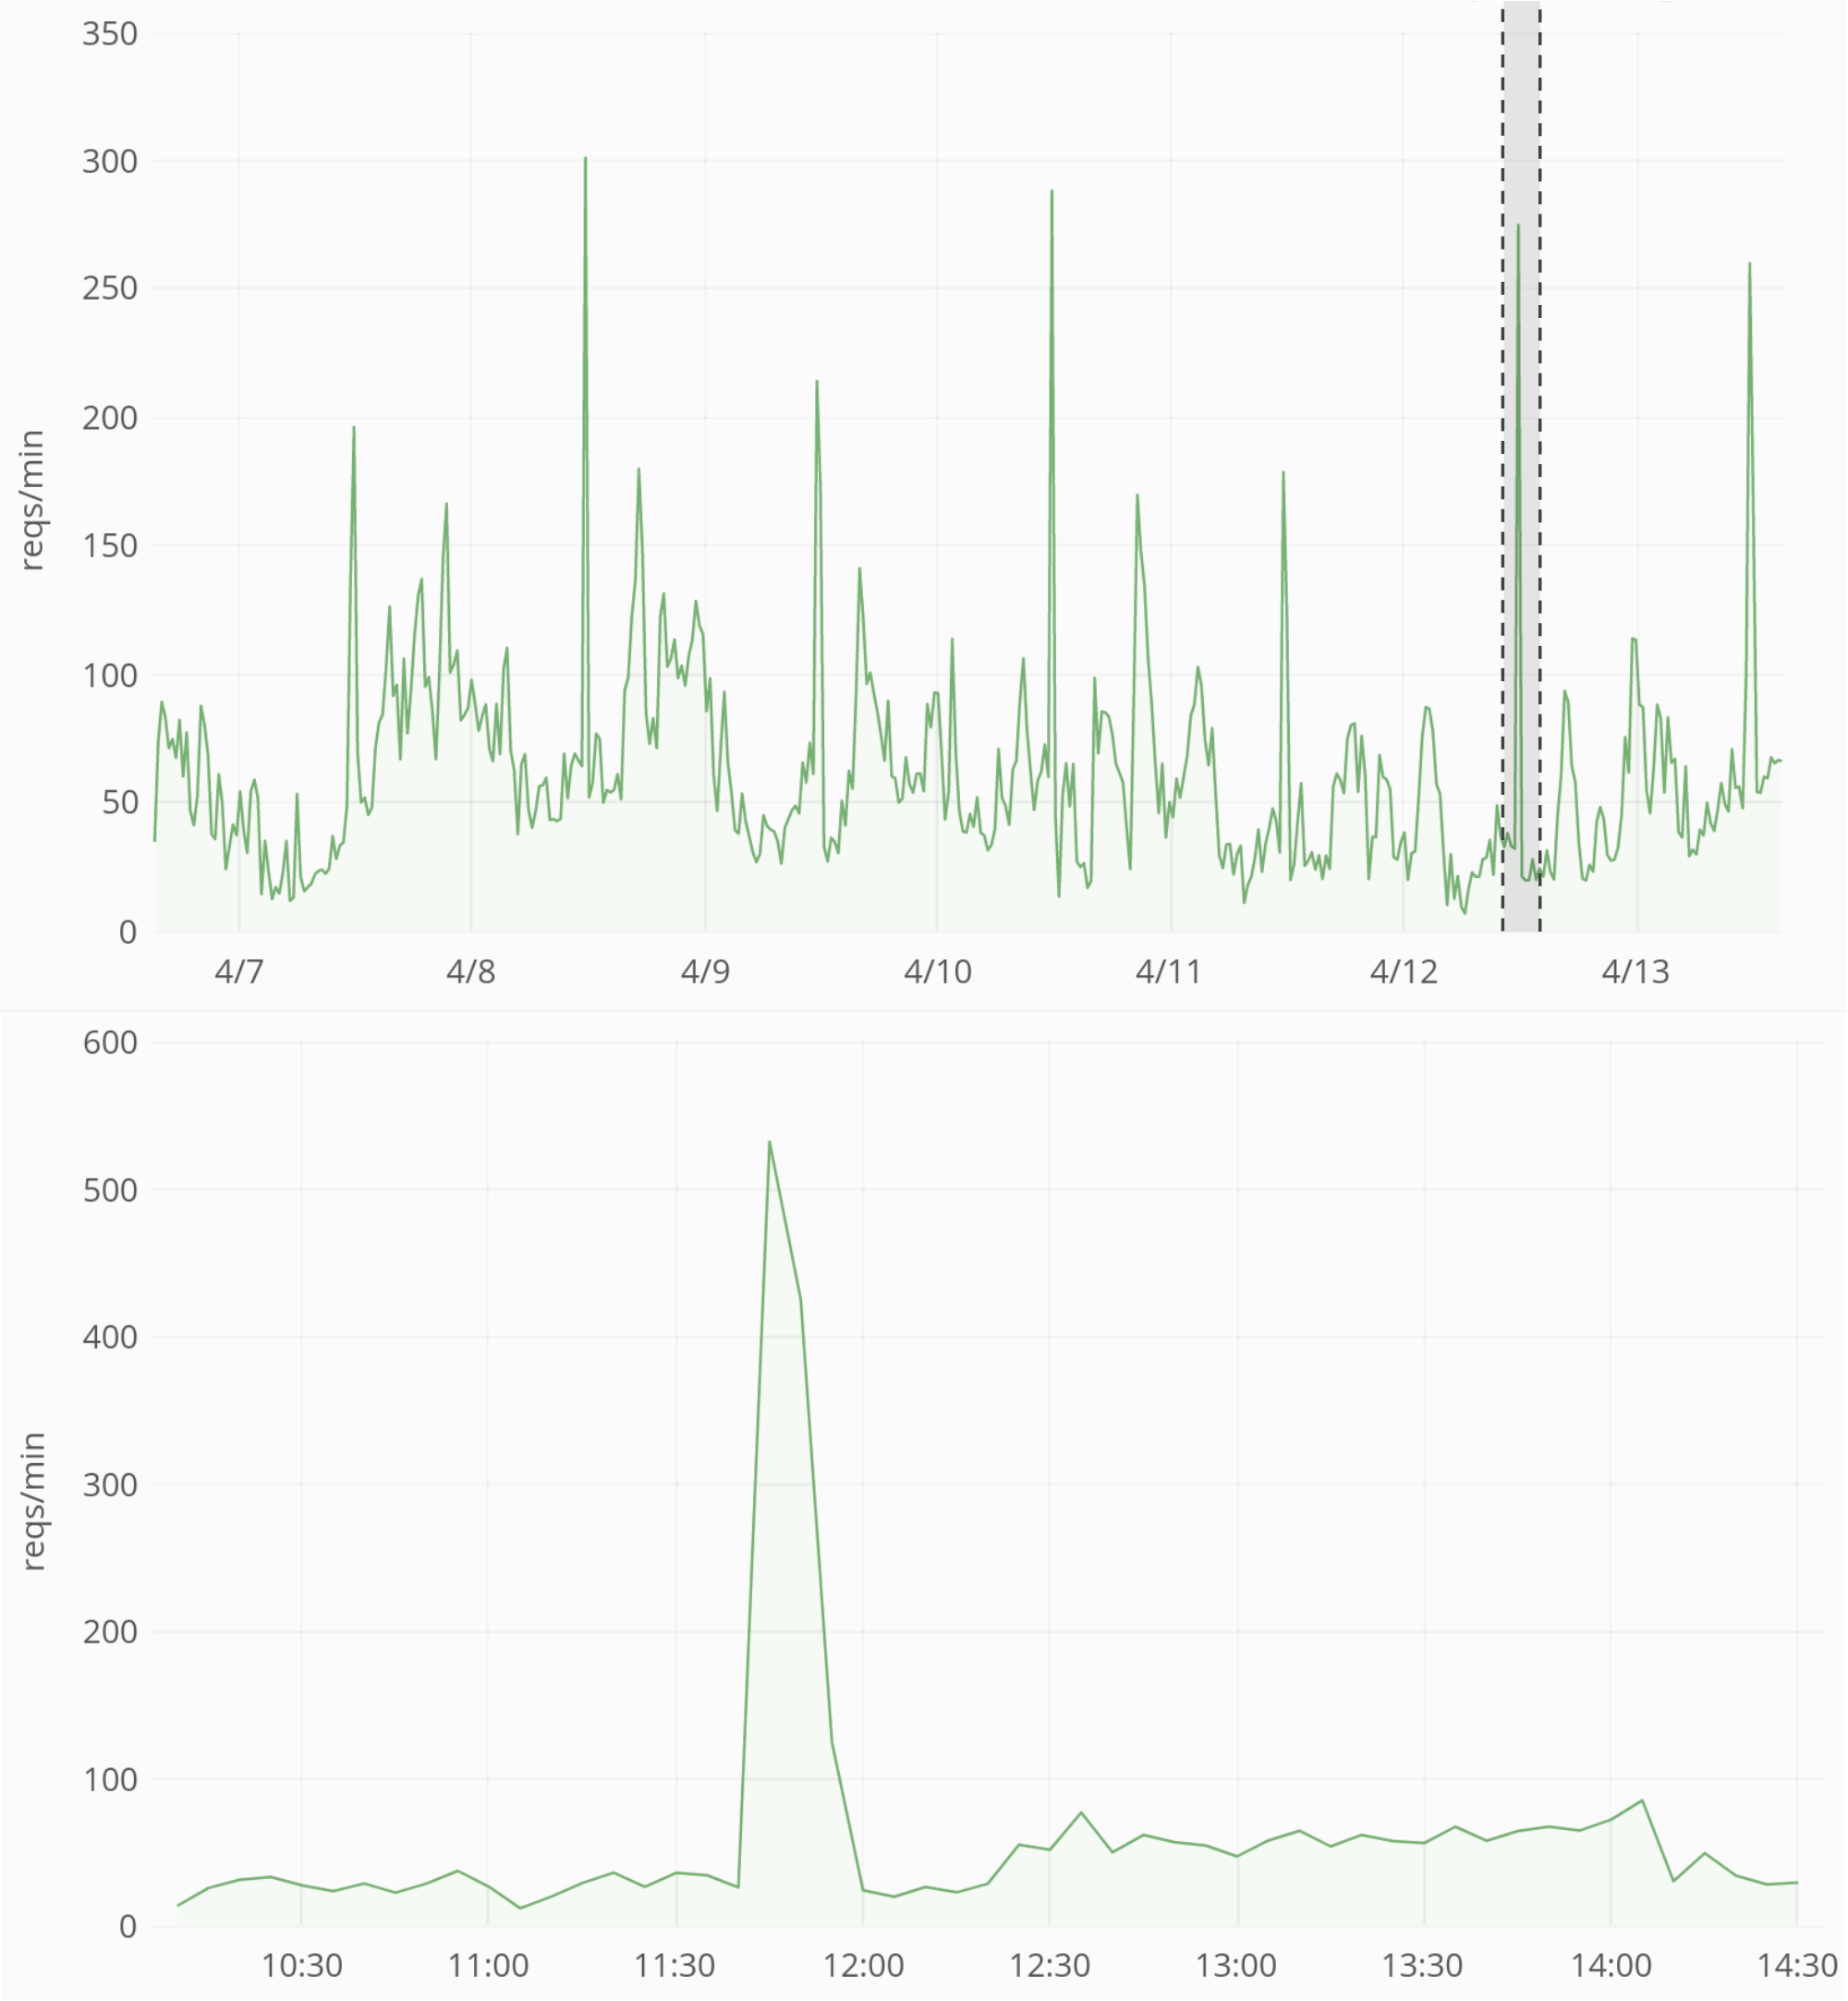
\includegraphics[width=.6\textwidth]{figures/ORES_request_activity_201804_week_vs_4hours}
  \caption{External requests per minute with a 4 hour block broken out to highlight a sudden burst of requests.}
  \label{fig:ores_request_rate}
\end{subfigure}\\
\begin{subfigure}[t]{\columnwidth}
  \centering
  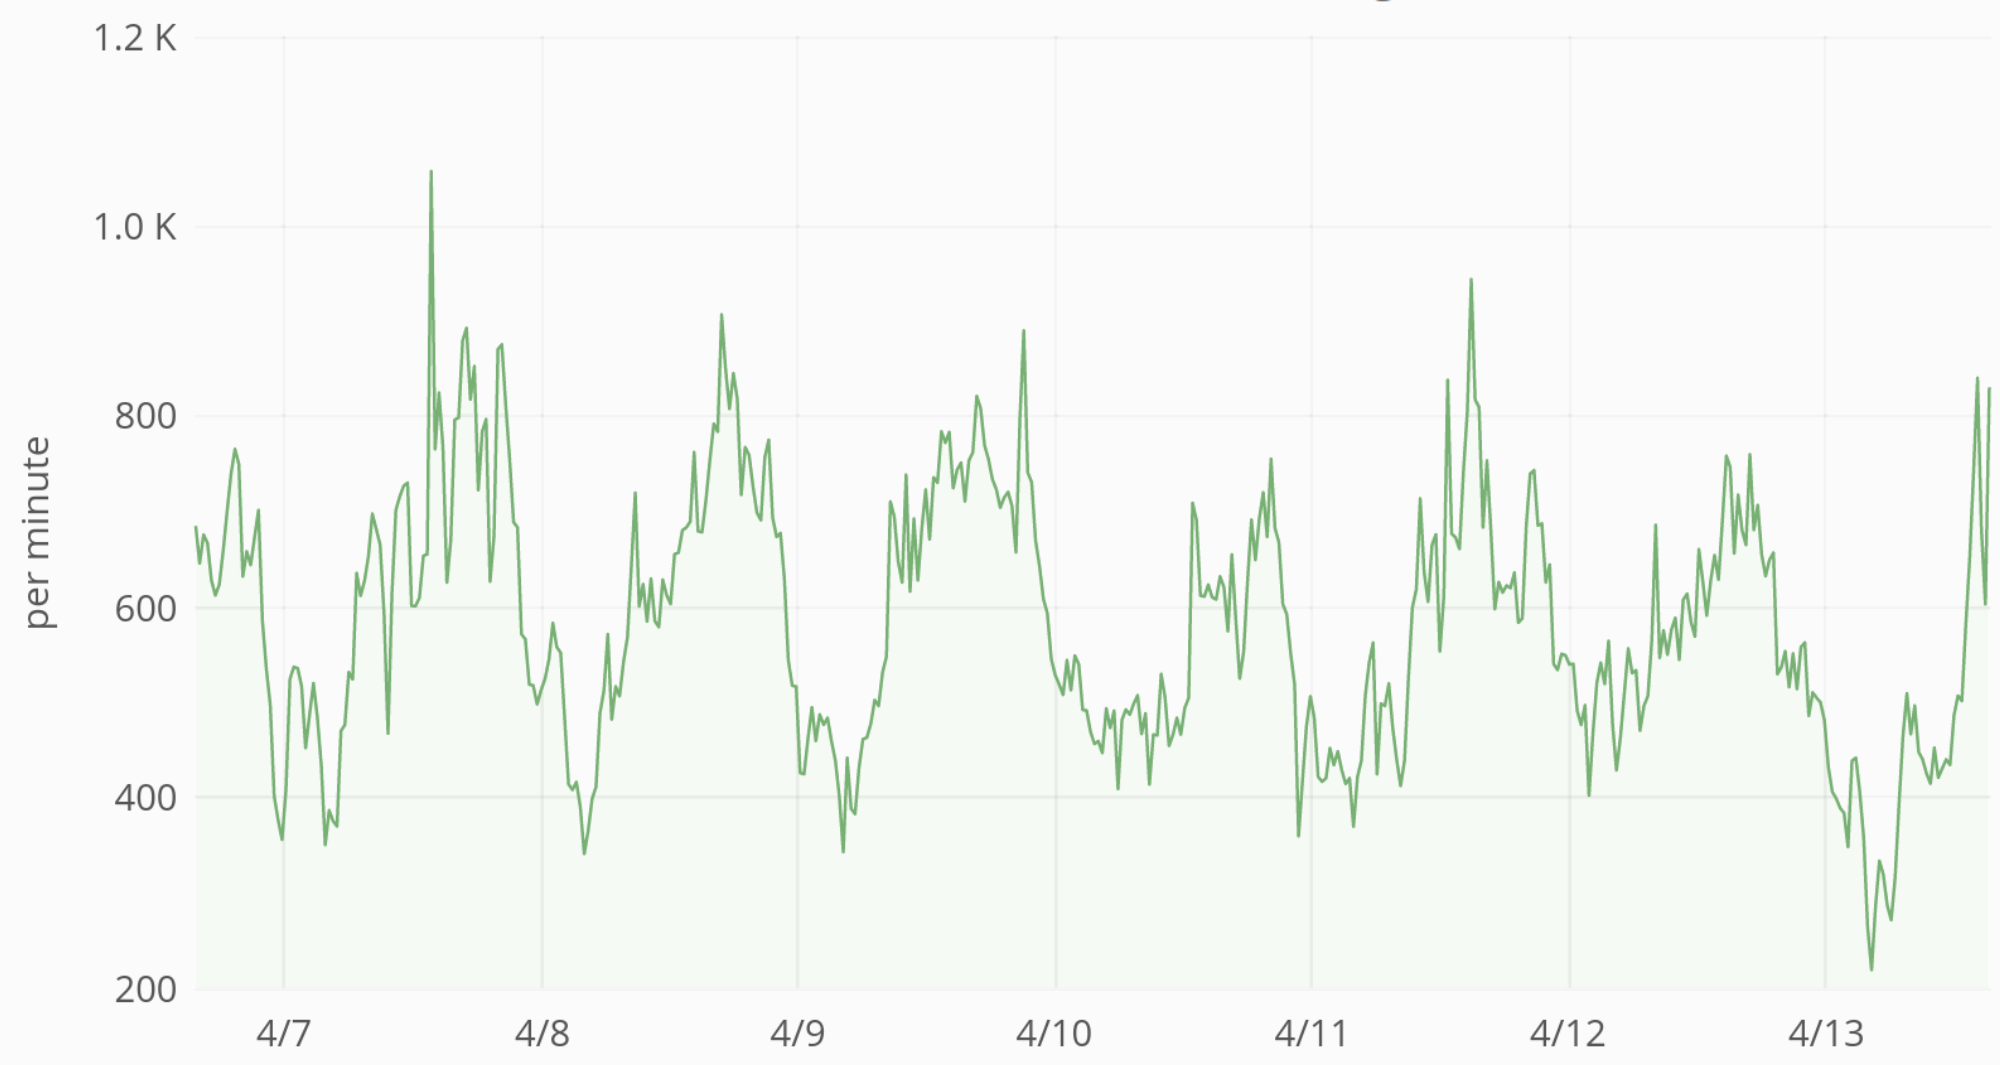
\includegraphics[width=.6\textwidth]{figures/ORES_precache_request_rate_201804}
  \caption{Precaching requests per minute}
  \label{fig:ores_precache_rate}
\end{subfigure}
\caption{Request rates to the ORES service for the week ending on April 13th, 2018}
\label{fig:ores_activity}
\end{figure*}


The ORES service has been online since July 2015\cite{halfaker2015artificial}.  Since then, usage has steadily risen as we've develop and deploy new models, and additional integrations are made by tool developers and researchers.  Currently, ORES supports 78 different models and 37 different language-specific wikis.

Generally, we see 50 to 125 requests per minute from external tools that are using ORES' predictions (excluding the MediaWiki extension that is more difficult to track).  Sometimes these external requests will burst up to 400-500 requests per second.  Figure~\ref{fig:ores_request_rate} shows the periodic and bursty nature of scoring requests received by the ORES service.  Note that every day at about 11:40 UTC, the request rate jumps---most likely a batch scoring job such as a bot.

Figure~\ref{fig:ores_precache_rate} shows our rate of precaching requests coming from our own systems.  This graph roughly reflects the rate of edits that are happening to all of the wikis that we support since we'll start a scoring job for nearly every edit as it happens.  Note that the number of precaching requests is about an order of magnitude higher than our known external score request rate.  This is expected, since Wikipedia editors and the tools they use will not request a score for every single revision.  This is a computational price we pay to attain a high cache hit rate and to ensure that our users get the quickest possible response for the scores that they \emph{do} need.

Taken together these strategies allow us to optimize the real-time quality control workflows and batch processing jobs of Wikipedians and their tools.  Without serious effort to make sure that ORES is practically fast and highly available to real-time use cases, ORES would become irrelevant to the target audience and thus irrelevant as a work-support infrastructure.  By engineering a system that conforms to the work-process needs of Wikipedians and their tools, we've built and systems intervention that has the potential gain wide adoption in Wikipedia's technical ecology. 


\section{Innovations in openness}
\label{sec:innovations_in_openness}
Our goals in the development of ORES and the deployment of models is to keep the process---the flow of data from random samples through model training and evaluation---open for review, critique, and iteration.  In this section, we'll describe how we implemented transparent reproducibility in our model development process, and how ORES outputs a wealth of useful and nuanced information for users.  By making this detailed information available to users and developers, we hope to enable flexibility and power in the evaluation and use of ORES predictions for novel purposes.

\subsection{Collaboratively labeled data}
There are two primary strategies for gathering labeled data for ORES' models: found traces and manual labels.

\leadin{Found traces.} For many models, there are already a rich set of digital traces that can be assumed to reflect a useful human judgement.  For example, in Wikipedia, it's very common that damaging edits will be reverted and that good edits will not be reverted.  Thus the revert action (and remaining traces) can be used to assume that the reverted edit is damaging.  We have developed a re-usable script\footnote{see \emph{autolabel} in \url{https://github.com/wiki-ai/editquality}} that when given a sample of edits, will label the edits as ``reverted\_for\_damage'' or not based on a set of constraints: edit was reverted within 48 hours, the reverting editor was not the same person, and the edit was not restored by another editor.

However, this ``reverted\_for\_damage'' label is problematic in that many edits are reverted not because they are damaging but because they are involved in some content dispute.  Also, the label does not differentiate damage that is a good-faith mistake from damage that is intentional vandalism.  So in the case of damage prediction models, we'll only make use of the ``reverted\_for\_damage'' label when manually labeled data is not available.

Another case of found traces is article quality assessments---named ``wp10'' after the Wikipedia 1.0 assessment where the article quality assessment scale originated\footnote{\url{http://enwp.org/WP:WP10}}.  We follow the process developed by Warncke-Wang et al.\cite{wang2017english} to extract the revision of an article that was current at the time of an assessment.  Many other wikis employ a similar process of article quality labeling (e.g. French Wikipedia and Russian Wikipedia), so we can use the same script to extract their assessments with some localization\footnote{see \emph{extract\_labelings} in \url{https://github.com/wiki-ai/articlequality}}.  However other wikis either do not apply the same labeling scheme consistently or at all and manual labeling is our only option.

\begin{figure}[h]
  \centering
  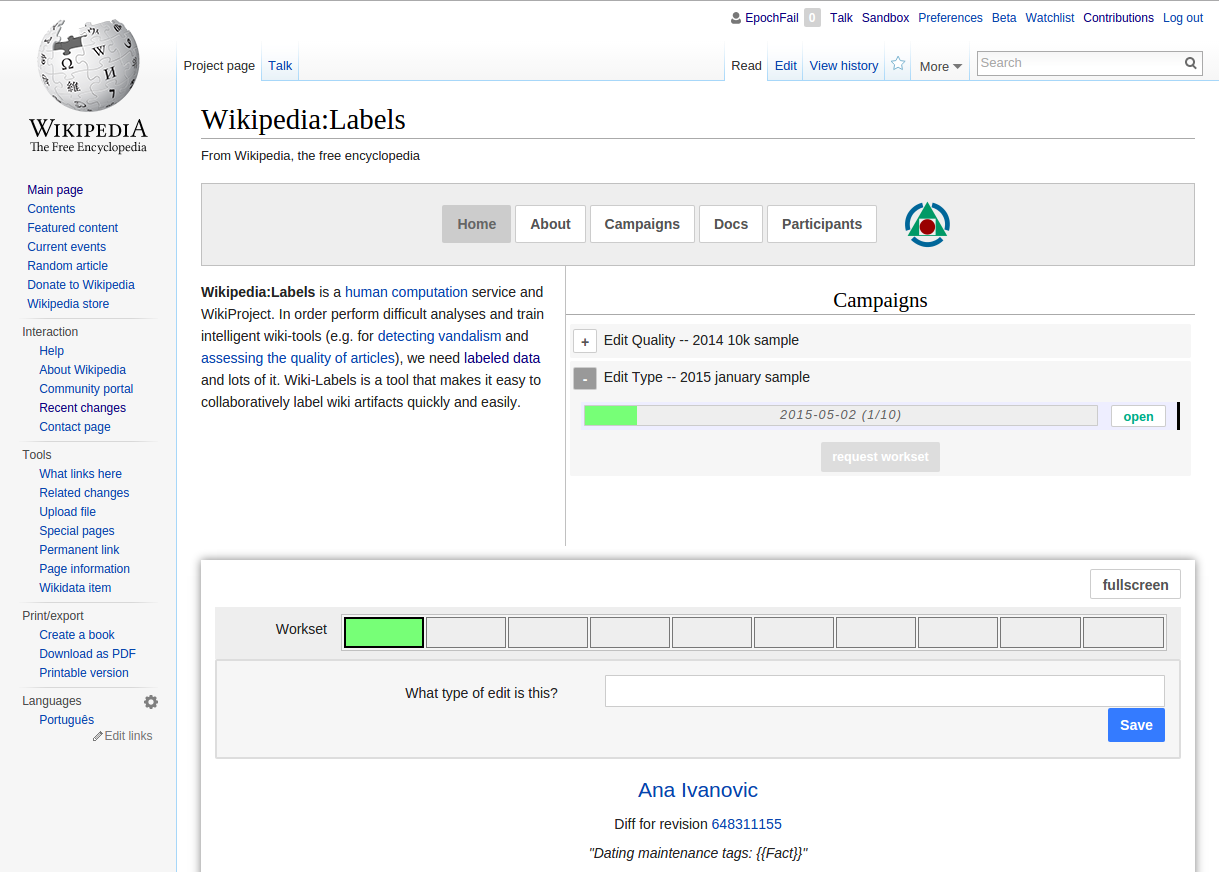
\includegraphics[width=.50\textwidth]{figures/Wiki_labels_gadget}
  \caption{The Wiki labels interface embedded in Wikipedia}
  \label{fig:wikilabels_screenshot}
\end{figure}

\leadin{Manual labeling.}
We hold manual labeling as the gold standard for purposes of training a model to replicate human judgement.  This contrasts with found data that is much easier to come by as it is available.  Manual labeling is an up-front expense of human labor.  In order to efficiently utilize valuable time investments by our collaborators, mostly volunteer Wikipedians, we've developed a system called ``Wiki Labels''\footnote{\url{http://enwp.org/:m:Wiki labels}}.  Wiki Labels allows Wikipedians to submit judgments of specific samples of Wiki content using a convenient interface and logging in via their Wikipedia account.

To supplement our models of edit quality, we replace the models based on found ``reverted\_for\_damage'' traces with manual judgments where we specifically ask labelers to distinguish ``damaging''/good from ``good-faith''/vandalism.  Using these labels we can build two separate models which allow users to filter for edits that are likely to be good-faith mistakes\cite{halfaker2017automated}, or just focus on vandalism, or to apply themselves broadly to all damaging edits.

We've managed to complete manual labeling campaigns for Turkish and Arabic Wikipedia article quality (wp10) as well as item quality in Wikidata.  We've found that, when working with manually labeled data, we can attain relatively high levels of fitness with 150 observations per quality class.

\subsection{Explicit pipelines}
One of our openness goals in training and deploying ORES prediction models is to make the whole data flow process understandable.  Consider the following code that represents a common pattern from our model-building Makefiles:
\begin{figure}[htbp]
        \makebox{\hrulefill}{
        \small
        \begin{verbatim}
datasets/enwiki.human_labeled_revisions.20k_2015.json:
        ./utility fetch_labels \
                https://labels.wmflabs.org/campaigns/enwiki/4/ > $@

datasets/enwiki.labeled_revisions.w_cache.20k_2015.json: \
                datasets/enwiki.labeled_revisions.20k_2015.json
        cat $< | \
        revscoring extract \
                editquality.feature_lists.enwiki.damaging \
                --host https://en.wikipedia.org \
                --extractor $(max_extractors) \
                --verbose > $@

models/enwiki.damaging.gradient_boosting.model: \
                datasets/enwiki.labeled_revisions.w_cache.20k_2015.json
        cat $^ | \
        revscoring cv_train \
                revscoring.scoring.models.GradientBoosting \
                editquality.feature_lists.enwiki.damaging \
                damaging \
                --version=$(damaging_major_minor).0 \
                (... model parameters ...)
                --center --scale > $@
        \end{verbatim}
        \hrule
        \normalsize}
        \caption{Makefile rules for English damage detection model.}
        \label{fig:english_damaging_makefile}
\end{figure}


Essentially, this code helps someone determine where the labeled data comes from (manually labeled via the Wiki Labels system).  It makes it clear how features are extracted (using the \texttt{revscoring extract} utility and the \texttt{enwiki.damaging} feature set).  Finally, this dataset of extracted features is used to cross-validate and train a model predicting the ``damaging'' label and a serialized version of that model is written to a file.  A user could clone this repository, install the set of requirements, and run \texttt{make enwiki\_models} and expect that all of the data-pipeline would be reproduced, and an exactly equivalent model obtained.

By explicitly using public resources and releasing our utilities and Makefile source code under an open license (MIT), we have essential implemented a turn-key process for replicating our model building and evaluation pipeline.  A developer can review this pipeline for issues knowing that they are not missing a step of the process because all steps are captured in the Makefile.  They can also build on the process (e.g. add new features) incrementally and restart the pipeline.  In our own experience, this explicit pipeline is extremely useful for identifying the origin of our own model building bugs and for making incremental improvements to ORES' models.

At the very base of our Makefile, a user can run \texttt{make models} to rebuild all of the models of a certain type.  We regularly perform this process ourselves to ensure that the Makefile is an accurate representation of the data flow pipeline.  Performing complete rebuild is essential when a breaking change is made to one of our libraries.  The resulting serialized models are saved to the source code repository so that a developer can review the history of any specific model and even experiment with generating scores using old model versions.

\subsection{Model information}
In order to use a model effectively in practice, a user needs to know what to expect from model performance.  E.g. how often is it that when an edit is predicted to be ``damaging'' it actually is? (\emph{precision}) or what proportion of damaging edits should I expect will be caught by the model? (\emph{recall})  The target metric of an operational concern depends strongly on the intended use of the model.  Given that our goal with ORES is to allow people to experiment with the use and reflection of prediction models in novel ways, we sought to build an general model information strategy.

\begin{figure}[htbp]
        \makebox{\hrulefill}{
        \small
        \begin{verbatim}
      "damaging": {
        "type": "GradientBoosting",
        "version": "0.4.0",
        "environment": {"machine": "x86_64", ...},
        "params": {center": true, "init": null, "label_weights": {"true": 10},
                   "labels": [true, false], "learning_rate": 0.01, "min_samples_leaf": 1,
                   ...},
        "statistics": {
          "counts": {"labels": {"false": 18702, "true": 743},
                     "n": 19445,
                     "predictions": {"false": {"false": 17989, "true": 713},
                                     "true": {"false": 331, "true": 412}}},
          "precision": {"labels": {"false": 0.984, "true": 0.34},
                        "macro": 0.662, "micro": 0.962},
          "recall": {"labels": {"false": 0.962, "true": 0.555},
                     "macro": 0.758, "micro": 0.948},
          "pr_auc": {"labels": {"false": 0.997, "true": 0.445},
                     "macro": 0.721, "micro": 0.978},
          "roc_auc": {"labels": {"false": 0.923, "true": 0.923},
                      "macro": 0.923, "micro": 0.923},
          ...
        }
      }
        \end{verbatim}
        \hrule
        \normalsize}
        \caption{Result of \url{https://ores.wikimedia.org/v3/scores/enwiki/?model_info&models=damaging}}
        \label{fig:english_damaging_model_info}
\end{figure}


The output captured in Figure~\ref{fig:english_damaging_model_info} shows a heavily trimmed JSON (human- and machine-readable) output of \emph{model\_info} for the ``damaging'' model in English Wikipedia.  Note that many fields have been trimmed in the interest of space with an ellipsis (``...'').  What remains gives a taste of what information is available.  Specifically, there is structured data about what kind of model is being used, how it is parameterized, the computing environment used for training, the size of the train/test set, the basic set of fitness metrics, and a version number so that secondary caches know when to invalidate old scores.  A developer using an ORES model in their tools can use these fitness metrics to make decisions about whether or not a model is appropriate and to report to users what fitness they might expect at a given confidence threshold.

\subsection{Score documents}
The predictions made by through ORES are also, of course, human- and machine-readable.  In general, our classifiers will report a specific prediction along with a set of probability (likelihood) for each class.  Consider article quality (wp10) prediction output in Figure~\ref{fig:english_damaging_model_info}.

\begin{figure}[htbp]
        \makebox{\hrulefill}{
        \small
        \begin{verbatim}
        "wp10": {
          "score": {
            "prediction": "Start",
            "probability": {
              "FA": 0.0032931301528326693, "GA": 0.005852955431273448,
              "B": 0.060623380484537165, "C": 0.01991363271632328,
              "Start": 0.7543301344435299, "Stub": 0.15598676677150375
            }
          }
        }
        \end{verbatim}
        \hrule
        \normalsize}
        \caption{Result of \url{https://ores.wikimedia.org/v3/scores/enwiki/34234210/wp10}}
        \label{fig:english_damaging_model_info}
\end{figure}

A developer making use of a prediction like this may choose to present the raw prediction ``Start'' (one of the lower quality classes) to users or to implement some visualization of the probability distribution across predicted classed (75\% Start, 16\% Stub, etc.).  They might even choose to build an aggregate metric that weights the quality classes by their prediction weight (e.g. Ross's student support interface\cite{ross2016visualizing} or the \emph{weighted sum} metric from \cite{halfaker2017interpolating}).

\subsection{Threshold optimization}
When we first started developing ORES, we realized that interpreting the likelihood estimates of our prediction models would be crucial to using the predictions effectively.  Essentially, the operational concerns of Wikipedia's curators need to be translated into a likelihood threshold.  For example, counter-vandalism patrollers seek catch all (or almost all) vandalism before it is allowed to stick in Wikipedia for very long.  That means they have an operational concern around the \emph{recall} of a damage prediction model.  They'd also like to review as few edits as possible in order to catch that vandalism.  So they have an operational concern around the \emph{filter rate}---the proportion of edits that are not flagged for review by the model\cite{halfaker2016notes}.

By finding the threshold of prediction likelihood that optimizes the filter-rate at a high level of recall, we can provide vandal-fighters with an effective trade-off for supporting their work.  We refer to these optimizations in ORES as \emph{threshold optimizations} and ORES provides information about these thresholds in a machine-readable format so that tools can automatically detect the relevant thresholds for their wiki/model context.

Originally, when we developed ORES, we defined these threshold optimizations in our deployment configuration.  But eventually, it became apparent that our users wanted to be able to search through fitness metrics to adapt their own optimizations.  Adding new optimizations and redeploying quickly became a burden on us and a delay for our users.  So we developed a syntax for requesting an optimization from ORES in realtime using fitness statistics from the models tests. E.g. \texttt{maximum recall @ precision >= 0.9} gets a useful threshold for a counter-vandalism bot or \texttt{maximum filter\_rate @ recall >= 0.75} gets a useful threshold for semi-automated edit review (with human judgement).

\begin{figure}[htbp]
        \makebox{\hrulefill}{
        \small
        \begin{verbatim}
  {"threshold": 0.299, ...,
   "filter_rate": 0.88, "fpr": 0.097, "match_rate": 0.12,
   "precision": 0.215, "recall": 0.751}
        \end{verbatim}
        \hrule
        \normalsize}
        \caption{Result of \url{https://ores.wikimedia.org/v3/scores/enwiki/?models=damaging&model_info=statistics.thresholds.true.'maximum filter_rate @ recall >= 0.75'}}
        \label{fig:english_damaging_threshold_optimization}
\end{figure}

This result shows that, when a threshold is set on 0.299 likelihood of damaging=true, then you can expect to get a recall of 0.751, precision of 0.215, and a filter-rate of 0.88.  While the precision is low, this threshold reduces the overall workload of vandal-fighters by 88\% while still catching 75\% of (the most egregious) damaging edits.

\subsection{Dependency injection and interrogability}
From a technical perspective, ORES is a algorithmic ``scorer'' container system.  It's primarily designed for hosting machine classifiers, but it is suited to other scoring paradigms as well.  E.g. at one point, our experimental installation of ORES hosted a Flesch-Kincaid readability scorer.  The only real constraints are that the scorer must express its inputs in terms of ``dependencies'' that ORES knows how to solve and the scores must be presentable in JSON (Javascript Object Notation).

\subsubsection{Dependency injection}
One of the key features of ORES that allows scores to be generated in an efficient and flexible way is a dependency injection framework.

\leadin{Efficiency.}
For example, there are several features that go into the ``damaging'' prediction model that are drawn from the \emph{diff} of two versions of an articles text (words added, words removed, badwords added, etc.)  Because all of these features ``depend'' on the \emph{diff}, the dependency solver can make sure that only one \emph{diff} is generated and that all subsequent features make use of that shared data.

ORES can serve multiple scores in the same request.  E.g. a user might want to gather a set of scores: ``edit type'', ``damaging'', and ``good-faith''.  Again, all of these prediction models depend on features related to the edit \emph{diff}.  ORES can safely combine all of the features required for each of the requested models and extract them with their shared dependencies together.  Given that feature extraction tends to take the majority of time in a real-time request request (partially for fetching data [IO], partially for computation time [CPU]), this allows the scoring for multiple, similar models to take roughly the same amount of time as scoring a single model.

\leadin{Flexibility.} When developing a model, it's common to experiment with different feature sets.  A natural progression in the life of a model in the wild involves the slow addition of new features that prove useful during experimentation.  By implementing a dependency system and a dependency solver, a model can communicate to ORES which features it needs and ORES can provide those features.  At no point does a model developer need to teach ORES how to gather new data.  All of the information needed for the solver to solve any given feature set is wrapped up in the dependencies.

\subsubsection{Interrogability}
The flexibility provided by the dependency injection framework let us implement a novel strategy for exploring \emph{how} ORES' models make predictions.  By exposing the features extracted to ORES users and allowing them to inject their own features, we can allow users to ask how predictions would change if the world were different.  Let's look at an example to demonstrate.  Let's say you wanted to explore how ORES judges unregistered (anon) editors differently from registered editors.


\begin{figure}[htbp]
        \makebox{\hrulefill}{
        \small
        \begin{verbatim}
        "damaging": {
          "features": {
            ...
            "feature.revision.user.is_anon": false,
            ...
          },
          "score": {
            "prediction": false,
            "probability": {
              "false": 0.938910157824447,
              "true": 0.06108984217555305
            }
          }
        }
        \end{verbatim}
        \hrule
        \normalsize}
        \caption{Result of \url{https://ores.wikimedia.org/v3/scores/enwiki/34234210/damaging?features}}
        \label{fig:english_damaging_features}
\end{figure}

This essentially means that the ``damaging'' prediction model concludes that the edit identified by the \emph{revision ID} of 34234210 is not damaging with 93.9\% confidence.  We can ask ORES to make a prediction about the exact same edit, but to assume that the editor was unregistered.

\begin{figure}[htbp]
        \makebox{\hrulefill}{
        \small
        \begin{verbatim}
        "damaging": {
          "features": {
            ...
            "feature.revision.user.is_anon": true,
            ...
          },
          "score": {
            "prediction": false,
            "probability": {
              "false": 0.9124151990561908,
              "true": 0.0875848009438092
            }
          }
        }
        \end{verbatim}
        \hrule
        \normalsize}
        \caption{Result of \url{https://ores.wikimedia.org/v3/scores/enwiki/34234210/damaging?features&feature.revision.user.is_anon=true}}
        \label{fig:english_damaging_features}
\end{figure}

If this edit were saved by an anonymous editor, ORES would still conclude that the edit was not damaging, but with less confidence (91.2\%).  By following a pattern like this for a single edit or a set of edits, we can get to know how ORES prediction models account for anonymity.

This is a very powerful tool for interrogating ORES.  Imagine being able to ask a law enforcement officer if they feel like they have probable cause for a search and then asking again how their answer would change if the suspect were black.

Interrogability isn't only useful for checking to see where ORES biases originate and what effects they have on predictions.  For example, Ross has started using our article quality prediction models (\emph{wp10}) as a method for suggesting work to new editors\footnote{\url{https://dashboard-testing.wikiedu.org}}.  By asking ORES to score a student's draft and then asking ORES to reconsider the predicted quality level of the article with \emph{one more header}, \emph{one more image} , or \emph{one more citation}, they've built an intelligent user interface that can automatically recommend the most productive development to the article---the change that will most likely bring it to a higher quality level.


\section{Adoption patterns}
\label{sec:adoption_patterns}
When we designed and developed ORES, we were targeting a specific problem---expanding the set values applied to the design of quality control tools to include recent a recent understanding of the importance of newcomer socialization.  We don't have any direct control of how developers chose to use ORES.  We hypothesize that, by making edit quality predictions available to all developers, we would lower the barrier to experimentation in this space.  It's clear that we lowered barriers to experimentation.  After we deployed ORES, we implemented some basic tools to showcase ORES, but we observed a steady adoption of our various prediction models by external developers in current tools and through the development of new tools\footnote{See complete list: \url{http://enwp.org/:mw:ORES/Applications}}.

\subsection{Showcase tools}
In order to showcase the utility of ORES, we developed a two simple tools to surface ORES predictions within MediaWiki---the wiki that powers Wikipedia: \emph{ScoredRevisions} and the \emph{ORES Review Tool}.

\textbf{ScoredRevisions}\footnote{\url{https://github.com/he7d3r/mw-gadget-ScoredRevisions}} is a javascript-based ``gadget'' that runs on top of MediaWiki.  When certain pages load in the MediaWiki interface (E.g. Special:RecentChanges, Special:Watchlist, etc.), the ScoredRevisions submits requests to the ORES service to score the edits present on the page.  The javascript then updates the page with highlighting based on ORES predictions.  Edits that are likely to be ``damaging'' are highlighted in red.  Edits that might be damaging and are worth reviewing are highlighted in yellow.  Other edits are left with the default background.

While this interface was excellent for displaying ORES potential, it had limited utility.  First, it was severely limited by the performance of the ORES system.  While ORES is reasonably fast for scoring a single edit, scoring 50-500 edits (the ranges that commonly appear on these pages) can take 30 seconds to 2 minutes.  So a user is left waiting for the highlighting to appear.  Because ScoredRevisions is only able to score edits after they are rendered, there was no way for a user to ask the system to filter edits ahead of time to only show edits that are likely to be damaging.  The user needed to visually filter the long lists based on highlighted rows.

\textbf{The ORES Review Tool}\footnote{\url{http://enwp.org/:mw:ORES_review_tool}} is a MediaWiki extension implemented in PHP.  It uses an offline process to score all recent edits to Wikipedia and to store those scores in a table for querying and quick access.  This tool implemented similar functionality to \emph{ScoredRevisions} but because it had pre-cached ORES scores in a table, it rendered highlights for likely damaging edits as soon as the page loaded. It enabled users to filter based on likely damaging edits.

We released the ORES Review Tool as a ``beta feature'' on Wikimedia wikis were we were able to develop advanced edit quality models.  The response was extremely positive.  Over 26k editors in Wikipedia had manually enabled the ORES Review Tool by April of 2017.  For reference, the total number of active editors across all languages of Wikipedia varies around 70k\footnote{\url{https://stats.wikimedia.org/EN/TablesWikipediansEditsGt5.htm}}, so this means that about a 3rd of active editors consciously chose to enable the feature.

\subsection{Adoption in current tools}
Many tools for counter-vandalism in Wikipedia were already available when we developed ORES.  Some of them made use of machine prediction (e.g. Huggle\footnote{Notably, Huggle adopted ORES prediction models soon after we deployed}, STiki, ClueBot NG), but most did not.  Soon after we deployed ORES, many developers that had not previously included their own prediction models in their tools were quick to adopt ORES.  For example, RealTime Recent Changes\footnote{\url{http://enwp.org/:m:RTRC}} includes ORES predictions along-side their realtime interface and FastButtons\footnote{\url{http://enwp.org/:pt:Wikipédia:Scripts/FastButtons}}, a Portuguese Wikipedia gadget, began displaying ORES predictions next to their buttons for quick reviewing and reverting damaging edits.

Other tools that were not targeted at counter-vandalism also found ORES predictions---specific that of \emph{article quality} (wp10)---useful.  For example, RATER\footnote{\url{http://enwp.org/::en:WP:RATER}}, a gadget for supporting the assessment of article quality began to include ORES predictions to help their users assess the quality of articles and SuggestBot\footnote{\url{http://enwp.org/User:SuggestBot}}\cite{cosley2007suggestbot}, a robot for suggesting articles to an editor, began including ORES predictions in their tables of recommendations.

\subsection{Development of new tools}
\begin{figure}[h]
  \centering
  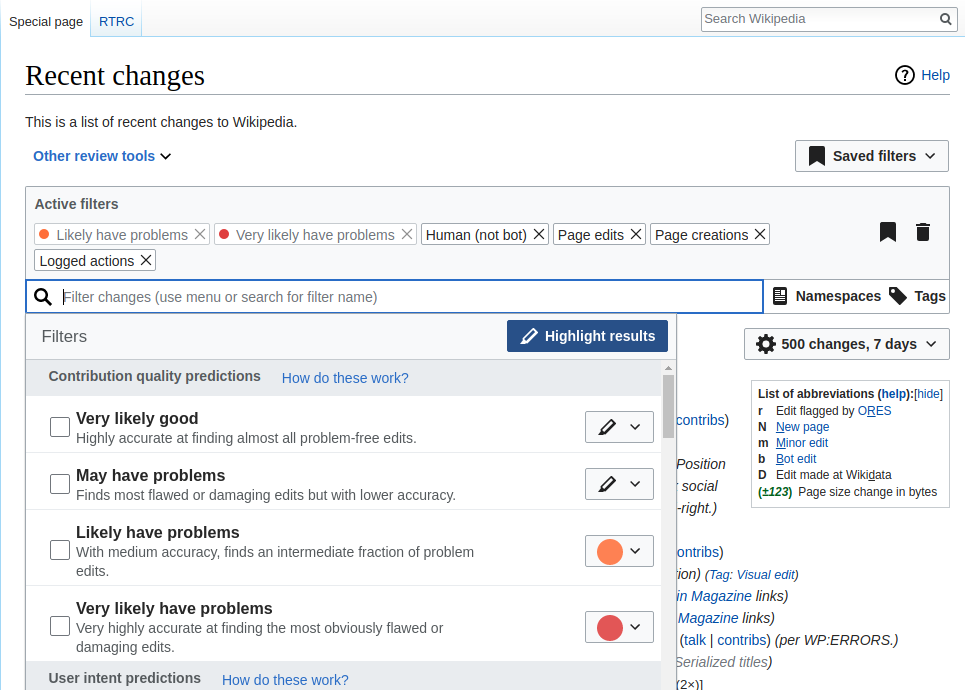
\includegraphics[width=.80\textwidth]{figures/Screenshot_of_Edit_review_filters}
  \caption{A screenshot of the Edit Review Filters interface with ORES score-based filters}
  \label{fig:edit_review_filters_screenshot}
\end{figure}

Many new tools have been developed since ORES has released that may not have been developed at all otherwise.  For example, the Wikimedia Foundation product department developed a complete redesign on MediaWiki's Special:RecentChanges interface that implements a set of powerful filters and highlighting.  They took the ORES Review Tool to it's logical conclusion with an initiative that they referred to as Edit Review Filters\footnote{\url{http://enwp.org/:mw:Edit_Review_Improvements}}.  In this interface, ORES scores are prominently featured at the top of the list of available features, and they have been highlighted as one of the main benefits of the new interface to the editing community.

When we first developed ORES, English Wikipedia was the only wiki that we are aware of that had a robot that used machine prediction to automatically revert obvious vandalism\cite{carter2008cluebot}.  After we deployed ORES, several wikis developed bots of their own to use ORES predictions to automatically revert vandalism.  For example, in PatruBOT in Spanish Wikipedia\footnote{\url{https://es.wikipedia.org/wiki/Usuario:PatruBOT}} and Dexbot in Persian Wikipedia\footnote{\url{https://fa.wikipedia.org/wiki/User:Dexbot}} now automatically revert edits that ORES predicts are damaging with high confidence.  These bots have been received with mixed acceptance.  Because of the lack of human oversight, concerns were raised about PatruBOT's false positive rate but after consulting with the developer, we were able to help them find an acceptable threshold of confidence for auto-reverts.

One of the most noteworthy new tools is the suite of tools developed by Sage Ross to support the Wiki Education Foundation's\footnote{\url{https://wikiedu.org/}} activities.  Their organization supports classroom activities that involve editing Wikipedia.  They develop tools and dashboards that help students contribute successfully and to help teachers monitor their students' work.  Ross has recently published about how they interpret meaning from ORES' article quality models\cite{ross2016visualizing} and has integrate this prediction into their tools and dashboards to recommend work that students need to do to bring their articles up to Wikipedia's standards.  See our discussion of interrogation in Section~\ref{sec:innovations_in_openness}.


\section{Case studies in reflection}
\label{sec:case_studies}
When we first deployed ORES, we reached out to several different wiki-communities and invited them to test out the system for use in patrolling for vandalism.  In these announcements, we encouraged editors to install ScoredRevisions,the only tool that used made use of ORES' edit quality models at the time.  ScoredRevisions both highlights edits that are likely to be damaging (as predicted by the model) and displays the likelihood of the prediction as a percentage.

Before long, our users began filing false-positive reports on wiki pages of their own design.  In this section we will describe three cases where our users independently developed these false-positive reporting pages and how they used them to understand ORES, the roles of automated quality control in their own spaces, and to communicate with us.

\subsection{Report mistakes (Wikidata)}
\begin{figure}[h]
  \centering
  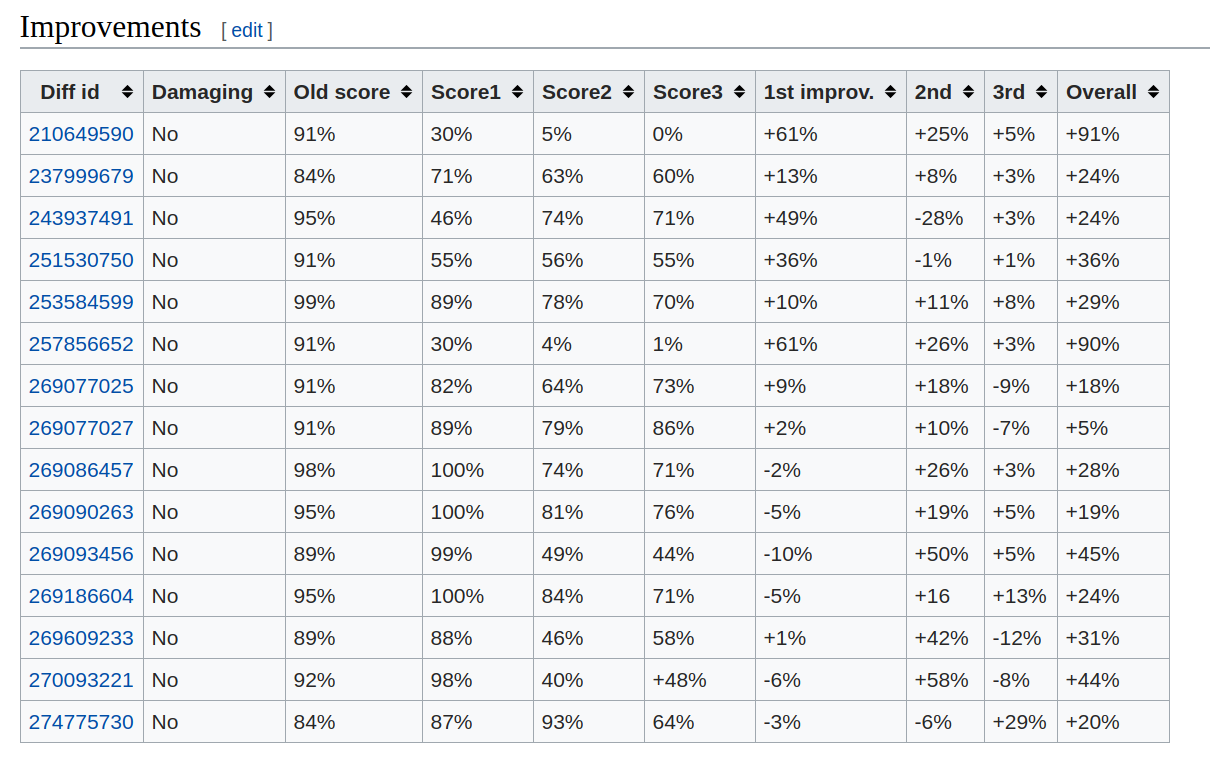
\includegraphics[width=.80\textwidth]{figures/ORES_report_mistakes_table}
  \caption{The ORES report mistakes table in Wikidata.}
  \label{fig:ores_report_mistakes}
\end{figure}

When we first deployed prediction models for Wikidata, a free and open knowledge base that can be read and edited by both humans and machines\footnote{\url{https://wikidata.org}}, we were breaking new ground by building a damage detection classifier based on a structured data wiki\cite{sarabadani2017building}.  So we created a page called ``Report mistakes'' and invited users to tell us about mistakes that the prediction model made on that page. We left the format and structure largely up to the users.

Within 20 minutes, we received our first report from User:Mbch that ORES was reporting edits that couldn't possibly be vandalism as potentially damaging.  As reports streamed in, we began to respond to them and make adjustments to the model building process to address data extraction bugs and to increase the signal so that the model differentiate damage from non-damaging edits.  After a month of reports and bug fixes, we decided to build a table to represent the progress that we made in iterations on the model against the reported false-positives.  See Figure~\ref{fig:ores_report_mistakes} for a screenshot of the table.  Each row represents a mis-classified edit, and each column describes the progress we made in not detecting those edits as damaging in future iterations of the model.  Through this process, we learned how Wikidata editors saw damage and how our modeling and feature extraction process captured signals in ways that differed from Wikidata editors' understandings.  We were also able to publicly demonstrate improvements to this community.

\subsection{Patrolling/ORES (Italian Wikipedia)}
Italian Wikipedia was one of the first wikis where we deployed basic edit quality models.  Our local collaborator who helped us develop the language specific features, User:Rotpunkt, created a page for ORES\footnote{\url{http://enwp.org/:it:Progetto:Patrolling/ORES}} with a section for reporting false-positives (``falsi positivi'').  Within several hours, Rotpunkt and a few other edits started to notice some trends in their false positive reports.  First, Rotpunkt noticed that there were several counter-vandalism edits that ORES was flagging as potentially damaging, so he made a section for collecting that specific type of mistake (``annullamenti di vandalismo'').  A few reports later and he added a section for ''corrections to the verb for \emph{have}'' (``correzioni verbo avere'').  Through this process, editors from Italian Wikipedia were essential performing a grounded theory exploration of the general classes of errors that ORES was making.

Once there were several of these mistake-type sections and several reports within each section, Rotpunkt reached out to us to let us know what he had found.  He explained to us (via our IRC channel) that many of ORES mistakes were understandable, but there were some general trends in mistakes around the Italian verb for \emph{have}: ``ha''.  We knew immediately what was likely to be the issue.  It turns out that ``ha'' in English and many other languages is laughing, an example of informal language that doesn't belong in an encyclopedia article.  While the word ``ha'' in Italian translates to ``have'' and is perfectly acceptable in articles.

Because of the work of Rotpunkt and his collaborators in Italian Wikipedia, we were able to recognize the source of this issue (a set of features intended to detect the use of \emph{informal language} in articles) and to remove ``ha'' from that list for Italian Wikipedia.  This is just one example of many issues we were able to address because of the grounded theory and thematic analysis performed by Italian Wikipedians.

\subsection{PatruBOT (Spanish Wikipedia)}
Soon after we released support for Spanish Wikipedia, User:jem developed a robot to automatically revert damaging edits using ORES predictions (PatruBOT).  This robot was not running for long before our discussion pages started to be bombarded with confused Spanish-speaking editors asking us questions about why ORES did not like their work.  We struggled to understand the origin of the complaints until someone reached out to us to tell us about PatruBOT and its activities.

We haven't been able to find the source code for PatruBot, but from what we've been able to gather looking at its activity, it appears to us that PatruBOT was too sensitive and was likely reverting edits that ORES did not have enough confidence about.  Generally, when running an automated counter-vandalism bot, the most immediately operational concern is around \emph{precision} (the proportion of positive predictions that are true-positives).  This is because mistakes are extra expensive when there's no human judgement between a prediction and a revert (rejection of the contribution).  The proportion of all damaging edits that are actually caught by the bot (\emph{recall}) is a secondary concern to be optimized.

We recommend that bot developers who are interested in running an automated counter-vandalism bot use a threshold that maximizes recall at high precision (90\% is a good starting point).  According to our queries\footnote{\url{https://ores.wikimedia.org/v3/scores/eswiki?models=damaging&model_info=statistics.thresholds.true.\%27maximum\%20recall\%20@\%20precision\%20\%3E=\%200.9\%27}}, the Spanish Wikipedia damaging model can be expected to have 90\% precision and catch 17\% of damage if the bot only reverted edits where the likelihood estimate is above 0.959.

We reached out to the bot developer to try to help, but given the voluntary nature of their work, they were not available to discuss the issue with us.  Eventually, other editors who were concerned with PatruBOT's behavior organized an informal crowdsourced evaluation of the fitness of PatruBOT's behavior\footnote{\url{http://enwp.org/:es:Wikipedia:Mantenimiento/Revisi\%C3\%B3n_de_errores_de_PatruBOT\%2FAn\%C3\%A1lisis}} where they randomly sampled 1000 reverts performed by PatruBOT and reviewed their appropriateness. At the time of writing, PatruBOT has been stopped\footnote{\url{http://enwp.org/:es:Wikipedia:Caf\%C3\%A9\%2FArchivo\%2FMiscel\%C3\%A1nea\%2FActual\#Parada_de_PatruBOT}} and the informal evaluation is ongoing.

\subsection{Bias against anonymous editors}
Shortly after we deployed ORES, we started receiving reports that ORES' damage detection models were overly biased against anonymous editors.  At the time, we were using LinearSVC\footnote{\url{http://scikit-learn.org/stable/modules/generated/sklearn.svm.LinearSVC.html}} estimators to build classifiers, and we were considering making the transition towards ensemble strategies like GradientBoosting and RandomForest estimators\footnote{\url{http://scikit-learn.org/stable/modules/ensemble.html}}.  We took the opportunity to look for bias in the error of estimation between anonymous editors, newly registered editors.  By using our feature injection/interrogation strategy(described in Section~\ref{sec:innovations_in_openness}), we could ask our current prediction models how they would change their predictions if the exact same edit were made by a different editor.

\begin{figure}[h]
\centering
\begin{subfigure}[t]{.33\textwidth}
  \centering
  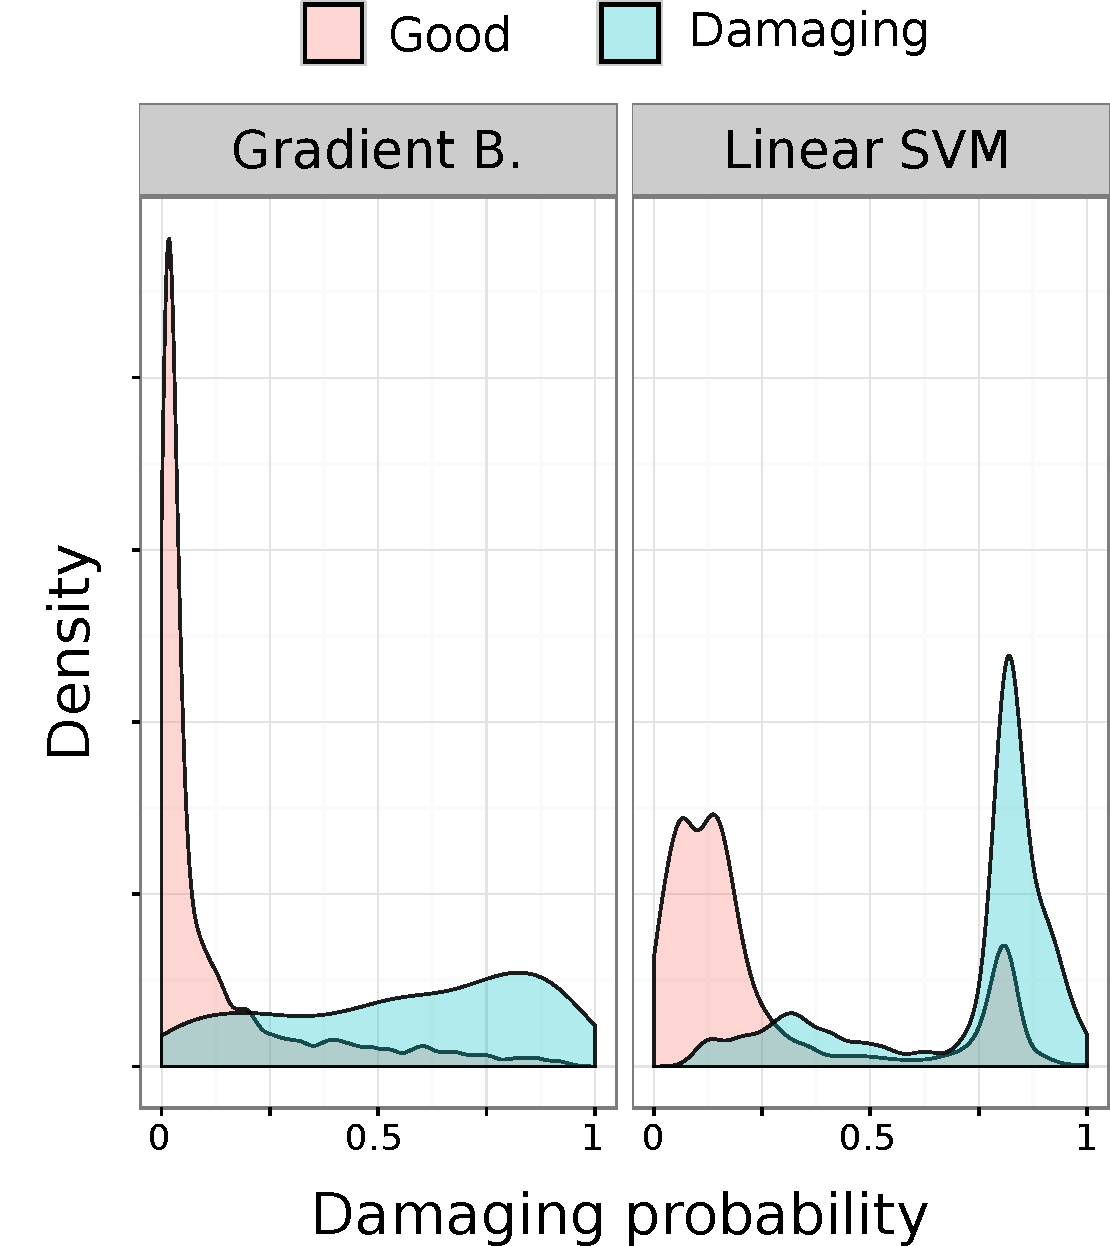
\includegraphics[width=.95\textwidth]{figures/natural_damaging_gb_vs_svc}
  \caption{No injected features}
  \label{fig:natural_damaging_gb_bs_svc}
\end{subfigure}~~
\begin{subfigure}[t]{.33\textwidth}
  \centering
  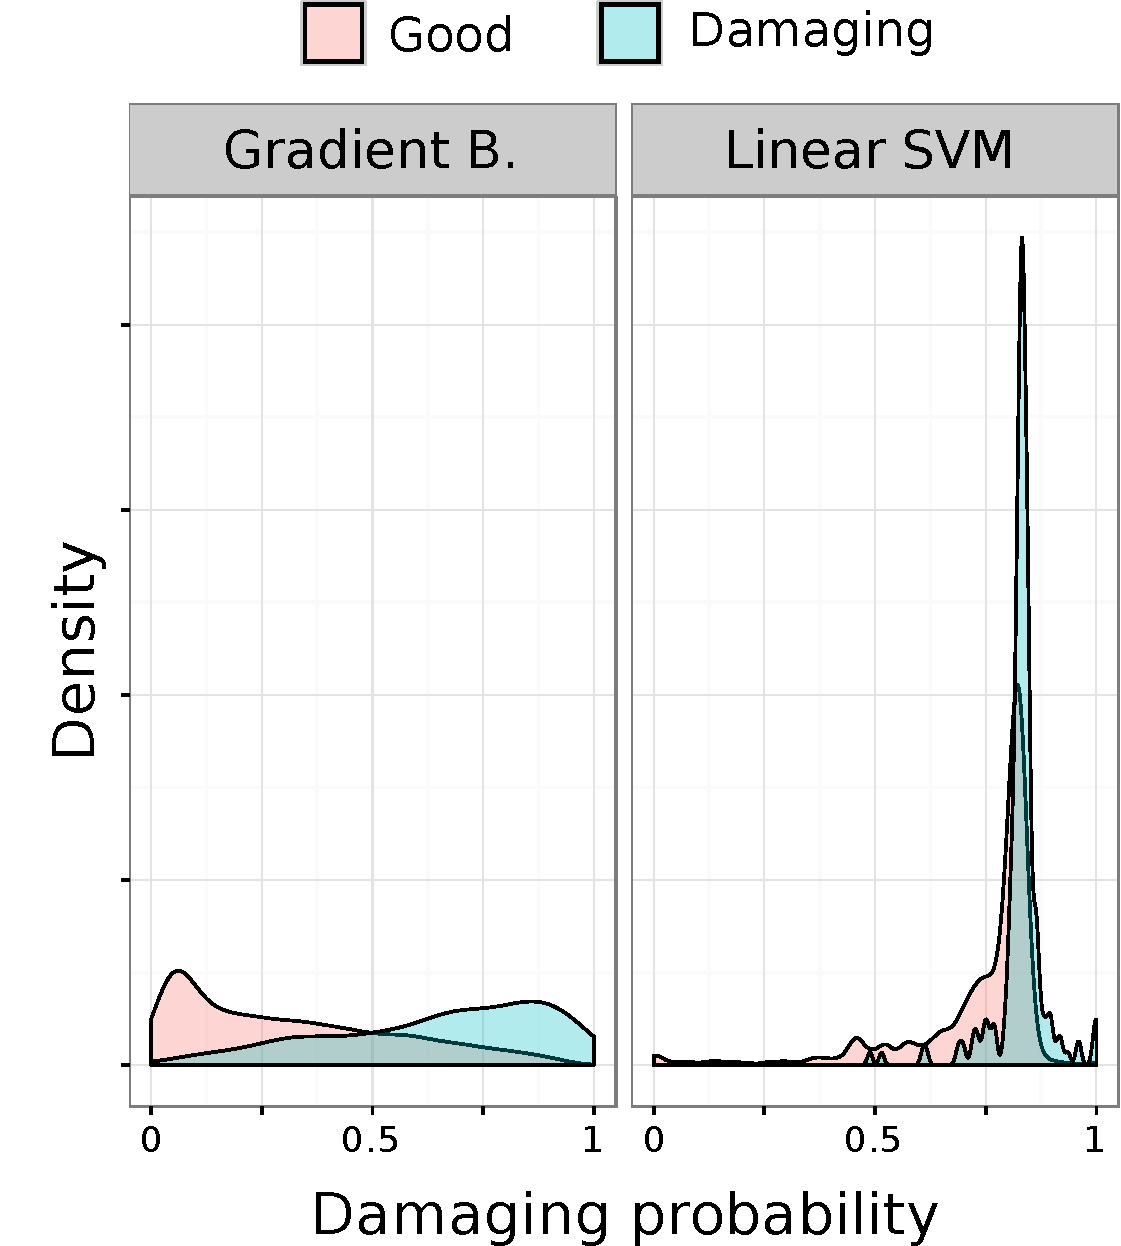
\includegraphics[width=.95\textwidth]{figures/anon_damaging_gb_vs_svc}
  \caption{Everyone is anonymous}
  \label{fig:anon_damaging_gb_bs_svc}
\end{subfigure}~~
\begin{subfigure}[t]{.33\textwidth}
  \centering
  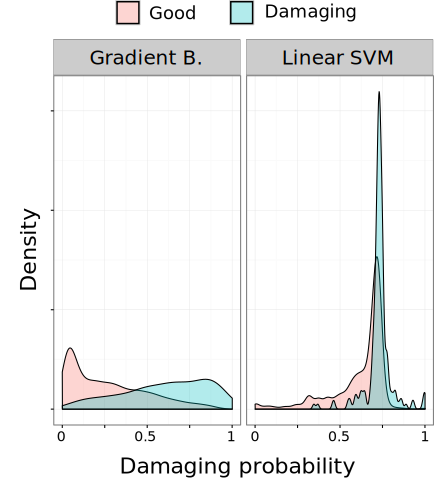
\includegraphics[width=.95\textwidth]{figures/newcomer_damaging_gb_vs_svc}
  \caption{Everyone is newly registered}
  \label{fig:newcomer_damaging_gb_bs_svc}
\end{subfigure}
\caption{The distributions of the probability of a single edit being scored as ``damaging'' based on injected features for the target user-class is presented.  Note that when injecting user-class features (anon, newcomer), all other features are held constant.}
\label{fig:prediction_error_for_anons_and_newcomers}
\end{figure}


Figure~\ref{fig:prediction_error_for_anons_and_newcomers} shows the probability density of the likelihood of ``damaging'' given three different passes over the exact same test set using two of our modeling strategies (``svc'' represents the old, LinearSVC strategy and ``gb'' represents the potential future GradientBoosting strategy).  Figure~\ref{fig:natural_damaging_gb_bs_svc} shows that, when we leave the features to their natural values, it appears that both models are able to differentiate effectively between damaging edits (high \emph{true\_proba}) and non-damaging edits (low \emph{true\_proba}) with the odd exception of a large amount of non-damaging edits with a relatively high \emph{true\_proba} around 0.8 in the case of the LinearSVC model.  Figures~\ref{fig:anon_damaging_gb_bs_svc} and \ref{fig:newcomer_damaging_gb_bs_svc} show a stark difference.  For the scores that go into these plots, characteristics of anonymous editors and newly registered editors were injected for all of the test edits.  We can see that the GradientBoosting model can still differentiate damage from non-damage while the LinearSVC model flags nearly all edits as damage in both case.

Through the reporting of this issue and our subsequent analysis, we were able to identify the issue and show that an improvement to our modeling strategy mitigates the problem.  Without such a tight feedback loop, we most likely wouldn't have noticed how poorly ORES' damage detection models were performing in practice.  Worse, it might have caused vandal-fighters to be increasingly (and inappropriately) skeptical of contributions by anonymous editors and newly registered editors---two groups of contributors that are already met with unnecessary hostility\footnote{\url{http://enwp.org/:en:Wikipedia:IPs_are_human_too}}\cite{halfaker2013rise}.

\subsection{Discussion}
These case studies in responses to ORES provide a window into how our team has been able to work with the locals in various communities to refine our understandings of their needs, into methods for recognizing and addressing biases in ORES' models, and into how people think about what types of automation they find acceptable in their \emph{spaces}.

\leadin{Refining our understandings and iterating our models.}
The information divide between us researchers/engineers and those members of a community is often wider than we realize.  Through iteration with the Wikidata and Italian models, we learned about incorrect assumptions we would made about how edits happen (e.g. client edits in Wikidata) and how language works (e.g. ``ha'' is not laughing in Italian).  It's likely we would never be able to fully understand the context in which damage detection models should operate before deploying the models.  But these case studies demonstrate how, with a tight communication loop, many surprising and wrong assumptions that were baked into our modeling process could be identified and addressed quickly.  It seems that many of the relevant issues in feature engineering and model tuning become apparent when the model is used in context to try to address a real problem (in these cases, counter-vandalism).

\leadin{Methods for recognizing and addressing bias.}
The Italian Wikipedians showed us something surprising and interesting about collaborative evaluation of machine prediction: thematic analysis is very powerful.  Through the collection of ORES mistakes and iteration, our Italian collaborators helped us understand general trends in the types of mistakes that ORES made.  It strikes us that this a somewhat general strategy for bias detection.  While our users certainly brought their own biases to their audit of ORES, they were quick to discover and come to consensus about trends in ORES' issues.  Before they had performed this process and shared their results with us, we had no idea that any issues was present.  After all, the fitness statistics for the damage detection model looked pretty good---probably good enough to publish a research paper!  Their use of thematic analysis seems to like a powerful tool that developers will want to make sure is well supported in any crowd based auditing support technologies.

\leadin{How people think about ``acceptable'' automation.}
In our case study, Spanish Wikipedians are in the processes of coming to agreements about what roles are acceptable for automated agents.  Through observation of PatruBOT's behavior, they have decided that the \emph{false discovery rate} (i.e., $1 - \text{precision}$) was too high by watching the bot work in practice and they started their own independent analysis to find quantitative, objective answers about what the real rate is.  Eventually they may come to a conclusion about an acceptable \emph{false discovery rate} or they may decide that no revert is acceptable without human intervention.


\section{Conclusion and future work}
\label{sec:conclusions_and_future_work}
Designing for empowerment leads us in new directions.  Rather than running an experiment on an ``intervention'' (e.g. \cite{halfaker2014snuggle}), we're reducing barriers and encouraging a stalled ``conversation'' continue.  We see this as a ``hearing to speech'' ala Nell Morten\cite{morton1985journey} in contrast to ``speaking to be heard''.  By building the exact technology or process we think is right, we would be ``speaking to be heard'' and forcing our own views into the technological conversation about how quality is enacted in Wikipedia.  By stepping back and asking, ``What is preventing others from getting involved in this conversation?'' and lowering those barriers, we run the risk that the conversation will not go in the directions that we value.  It is a conscious choice we make to attempt to empower others rather than to assert ourselves, but we do not make this choice purely out of altruism.  It is impractical for one individual or small group to drive a conversation in Wikipedia in a productive direction.  Halfaker et al.'s Snuggle intervention\cite{halfaker2014snuggle} tried that strategy with limited success in past work.  We think it's time to hear to speech and see what others would like to contribute from their own standpoints.

When considering our design rationale, ORES is not quite a successor system.  It doesn't directly enact an alternative vision of how quality control should function in Wikipedia  It is a system for making the construction of successor technologies easier.  By solving for efficiency and letting others design for process, a new set of expanded standpoints can more easily be expressed.  Under another view, ORES is maybe a successor in that it enacts an alternative view of how algorithms should be made available to the populations they govern.  By keeping algorithms integrated into specific tools and keeping the operational details of the algorithm hidden, past developers enacted values of control and focused use of their creations.  By opening ORES as an algorithmic system, encouraging experimentation, and providing tools for interrogation of the algorithms themselves, we enact a set of values that embrace experimentation and the progress of mediation.

We do intend to help Wikipedia's social process form in ways that align with our values---the more complete balance of efficient quality control and newcomer support.  We want to see Wikipedia work better. By ``better'' we mean that more people who want to contribute will feel welcome to do so and will find their place in Wikipedia.  In this paper we provide no direct evaluation of newcomer retention, nor do we look for evidence of improved newcomer socialization.  Instead, we're targeting the early precursors of social change: ecological health and critical reflection.  

\subsection{Ecological health}
In section~\ref{sec:adoption_patterns}, we show clear evidence of a boom in the ecosystem of quality control technologies.  Through the adoption of ORES, new tools have quickly gained relevant.  Many of these tools re-mediate the way that quality control happens in Wikipedia.  For example, Sage Ross's use of ORES' interrogability to support newcomers in developing articles that Wikipedians would find acceptable.  By using a quality model to direct newcomers behavior socialization may be improves at no cost to efficiency -- maybe even an improvement from a reviewer's point of view!  This addition to the technological conversation around quality control represents a substantial shift from the focus on the boundary\cite{geiger12socialization} to a focus on a pre-review training. 

\subsection{Critical reflection}
In section~\ref{sec:case_studies}, we show evidence of critical reflection on the current processes and the role of algorithms in quality control.  We believe that the case studies that we describe both show that this reflection is taking place and that the wide proliferation of tools that provide surprising alternative uses of ORES suggest that Wikipedians feel a renewed power over the their quality control processes.  Even if we are wrong about the direction of change that Wikipedia needs for quality control and newcomer socialization, we're inspired by much of the concern that has surfaced for looking into biases in ORES' prediction models (e.g. anons and the Italian ``ha'') and over what role algorithmis should have in directly reverting human actions (e.g. PatruBOT and DexBot).  Because of ORES' open API and Wikipedia's collaborative wiki pages, it was relatively straightforward for Wikipedians to audit ORES' predictions and collaborate with each other to build information about trends in ORES' mistakes and how they expected their own processes to function.

\subsection{Future work}
One of the clear lines of future work that observing ORES in the world drives us toward is improved crowd-based auditing tools.  As our case studies suggest, auditing of ORES' predictions and mistakes has become a very popular activity.  Despite the difficulty for a user of finding a deep wiki page and using templates to flag false positives, Wikipedians have managed to organize several similar processes for flagging false positives and calling them to our attention.  To better facilitate this process, future system builders should implement structured means to refute, support, discuss, and critique the predictions of machine models.  With a structured way to report false positives and other real-human judgments, we can make it easy for tools that use ORES to also allow for reporting mistakes.  We can also make it easier to query a database of ORES mistakes in order to build the kind of thematic analyses that Italian Wikipedians showed us.  By supporting such an activity, we are working to transfer more power from ourselves and to our users.  Should one of our models develop a nasty bias, our users will be more empowered to coordinate with each other, show that the bias exists and where it causes problems, and either get the model's predictions turned off or even shut down ORES.

We look forward to what those who work in the space of critical algorithm studies will do with ORES.  As of writing, most of the studies and critiques of \emph{subjective algorithms}\cite{tufekci2015algorithms} focus on large for-profit organizations like Google and Facebook---organizations that can't afford to open up their proprietary algorithms due to competition.  Wikipedia is one of the largest and most important information resources in the world.  The algorithms that ORES makes available are part of the decision process for allowing some people to contribute and preventing other.  This is a context where \emph{algorithms matter to humanity}, and we are openly experimenting with the kind of transparent and open processes that the \emph{fairness and transparency} researchers are advocating.  Yet we have new problems and new opportunities.  There is a large body of work exploring how biases manifest and how unfairness can play out in algorithmically mediated social contexts.  ORES would be an excellent place to expand the literature within a real and important field site.

Finally, we also see potential in allowing Wikipedians, the denizens of Wikipedia, to freely train, test, and use their own prediction models.  Currently, ORES is only suited to deploy models that are developed by someone with a strong modeling and programming background.  That doesn't need to be the case.  We have been experimenting with demonstrating ORES model building processes using Jupyter Notebooks\footnote{\url{http://jupyter.org}}\footnote{e.g. \url{ https://github.com/wiki-ai/editquality/blob/master/ipython/reverted_detection_demo.ipynb}} and have found that beginning programmers can understand the work involved.  This is still not the holy grail of crowd develop machine prediction---where all of the incidental complexities involved in programming are removed from the process of model development and evaluation.  Future work exploring strategies for allowing end-users to build models that are deployed by ORES would be a very interesting exploration of both the HCI issues involved and the changes the the technological conversations that such a margin-opening intervention might provide.


\section{Acknowledgements}
\label{sec:acknowledgements}
REDACTED FOR REVIEW


% Bibliography
\bibliographystyle{ACM-Reference-Format}
\bibliography{refs}


\end{document}
